\documentclass[instructions]{uqthesis}
%\documentclass[final]{uqthesis} 


%*************************************
% FOR YOUR FINAL THESIS
%*************************************

%IMPORTANT! 
%The default document class (above - line 1 & 2) for the template is \documentclass[instructions]{uqthesis} - this document class will show instructional material and examples relevant to the preliminary material in the compiled PDF preview. THESE INSTRUCTIONS ARE FOR YOUR REFERENCE ONLY AND ARE NOT TO BE INCLUDED IN YOUR FINAL THESIS! 

%To turn off these instructions in your final thesis you MUST use the document class \documentclass[final]{uqthesis} 
%To activate the final thesis document class you must UN-COMMENT THIS DOCUMENT CLASS (remove the % from the start of line 2) and comment out the instructional document class on line 1 (add % to the start of line 1). 


% ***************************************************
% LaTeX Packages
% ***************************************************
% This file defines the document design.
% Usually it is not necessary to edit this file, but you can use it to change aspects of the design if you want.

%There are essential packages that are contained within the uqthesis.cls which are integral to the template - These must not be deleted.  A list of these packages can be found in the README.tet file

%The packages below are optional, please add or alter as required.

\usepackage{cite}				 %Allows abbreviated numerical citations.
\usepackage{pdfpages}			 %Allows you to include full-page pdfs.
\usepackage{wrapfig}			 %Lets you wrap text around figures.
\usepackage{bm} 				 %Bolded maths characters.
\usepackage{upgreek}			 %Upright Greek characters.
\usepackage{dsfont}				 %Double-struck fonts.
\usepackage{simplewick}			 %For typesetting Wick contractions.
\usepackage{mathtools}		     %Can be used to fine-tune the maths presentation.	
\usepackage{framed}			     %For boxed text.
\usepackage{microtype}			 %pdfLaTeX will fix your kerning.
\usepackage{marvosym}			 %Include symbols (like the Euro symbol, etc.).
\usepackage{color}				 %Nice for scalable pdf graphics using InkScape.
\usepackage{transparent}	     %Nice for scalable pdf graphics using InkScape.
\usepackage{placeins}			 %Lets you put in a \FloatBarrier to stop figures floating past this command.
\usepackage{mdframed,mdwlist}    %Use these for nice lists (less white space).
\usepackage{graphicx}            %Enhanced support for graphics.
\usepackage{float}               %Improved interface for floating objects. 
\usepackage{longtable}           %Allow tables to flow over page boundaries.
\usepackage{mathdots}            %Changed the basic LaTeX and plain TeX commands.
\usepackage{eucal}               %Font shape definitions to use the Euler script symbols in math mode.
\usepackage{array}               %Extending the array and tabular environments.
\usepackage{stmaryrd}            %The StMary’s Road symbol font.
\usepackage{amsthm}              %St Mary Road symbols for theoretical computer science. 
\usepackage{pifont}              %Access to PostScript standard Symbol and Dingbats fonts.
\usepackage{lipsum}              %Easy access to the Lorem Ipsum dummy text.
\usepackage{enumerate}           %Enumerate with redefinable labels. 
\usepackage[all]{xy}             %This is a special package for drawing diagrams.
\usepackage{amsmath}             %ATypesetting theorems (AMS style).
\usepackage{amssymb}             %Provided an extended symbol collection.
\usepackage[utf8]{inputenc}      %Allowed all displayable utf8 characters to be available as input.
\usepackage{fancyhdr}            %Extensive control of page headers and footers.
\usepackage{blindtext}           %Produced 'blind' text for testing.
\usepackage{tikz}                %To create graphic elements.
\usepackage[figuresright]{rotating}	%Allows large tables to be rotated to landscape.
\usepackage{makecell}
\usepackage{tabularx}
\usepackage{listings}
\usepackage{bytefield}
\usepackage[most]{tcolorbox}
\usepackage{gensymb}
\usepackage{pgfplots}
\usepackage{subcaption}

\usepackage{booktabs}
\usepackage{multirow}

\usetikzlibrary{fit, patterns, positioning} % Import the fit library

\usetikzlibrary{shapes.geometric, arrows}
%You can add more packages here if you need


%This defines some macros that implement Latin abbreviations
%COMMENT OUT OR DELETE IF UNDESIRED.
\newcommand{\via}{\textit{via}} %Italicised via.
\newcommand{\ie}{\textit{i.e.}} %Literally.
\newcommand{\eg}{\textit{e.g.}} %For example.
\newcommand{\etc}{\textit{etc.}} %So on...
\newcommand{\vv}{\textit{vice versa}} %And the other way around.
\newcommand{\viz}{\textit{viz}.} %Resulting in.
\newcommand{\cf}{\textit{cf}.} %See, or 'consistent with'.
\newcommand{\apr}{\textit{a priori}} %Before the fact.
\newcommand{\apo}{\textit{a posteriori}} %After the fact.
\newcommand{\vivo}{\textit{in vivo}} %In the flesh.
\newcommand{\situ}{\textit{in situ}} %On location.
\newcommand{\silico}{\textit{in silico}} %Simulation.
\newcommand{\vitro}{\textit{in vitro}} %In glass.
\newcommand{\vs}{\textit{versus}} %James \vs{} Pete.
\newcommand{\ala}{\textit{\`{a} la}} %In the manner of...
\newcommand{\apriori}{\textit{a priori}} %Before hand.
\newcommand{\etal}{\textit{et al.}} %And others, with correct punctuation.
\newcommand{\naive}{na\"\i{}ve} %Queen Amidala is young and \naive{}.

\lstset{
  language=C,                          % Choose the language
  basicstyle=\ttfamily\footnotesize,    % Set the basic style (smaller)
  keywordstyle=\color{blue},            % Set keyword style
  commentstyle=\color{green},           % Set comment style
  stringstyle=\color{red},              % Set string literal style
  directivestyle=\color{magenta},       % Set directive style (for #define, etc.)
  numbers=left,                         % Where to put line numbers
  numberstyle=\tiny\color{gray},        % Line number style
  stepnumber=1,                         % Step between line numbers
  showstringspaces=false,               % Don't emphasize spaces in strings
  breaklines=true,                      % Break long lines
  frame=single,                         % Frame code
  captionpos=b, 
  rulecolor=\color{black}               % Rule/frame color
}


\lstset{
  language=VHDL,                          % Choose the language
  basicstyle=\ttfamily\footnotesize,    % Set the basic style (smaller)
  keywordstyle=\color{blue},            % Set keyword style
  commentstyle=\color{green},           % Set comment style
  stringstyle=\color{red},              % Set string literal style
  directivestyle=\color{magenta},       % Set directive style (for #define, etc.)
  numbers=left,                         % Where to put line numbers
  numberstyle=\tiny\color{gray},        % Line number style
  stepnumber=1,                         % Step between line numbers
  showstringspaces=false,               % Don't emphasize spaces in strings
  breaklines=true,                      % Break long lines
  frame=single,                         % Frame code
  captionpos=b, 
  rulecolor=\color{black}               % Rule/frame color
}

\lstdefinestyle{consoleoutput}{
    basicstyle=\small\ttfamily,
    breaklines=true,
    frame=single,
    backgroundcolor=\color[gray]{0.9}
}


\definecolor{lightergray}{gray}{0.95}
\newcommand{\codebg}[1]{\colorbox{lightergray}{\lstinline!#1!}}

\newcommand{\memsection}[4]{
    \bytefieldsetup{bitheight=#3\baselineskip}
    \bitbox[]{10}{
    \texttt{#1}% print end address
    \\
    % do some spacing
    \vspace{#3\baselineskip}
    \vspace{-2\baselineskip}
    \vspace{-#3pt}
    \texttt{#2}% print start address
    }%
    \bitbox{16}{#4}% print box with caption
}

\newcommand{\memsectioncolour}[4]{
    \bytefieldsetup{bitheight=#3\baselineskip}
    \bitbox[]{10}{
    \texttt{#1}% print end address
    \\
    % do some spacing
    \vspace{#3\baselineskip}
    \vspace{-2\baselineskip}
    \vspace{-#3pt}
    \texttt{#2}% print start address
    }%
    \bitbox{16}[bgcolor=lightergray]{#4}% print box with caption
}


\setcounter{secnumdepth}{4}


% ***************************************************
% Title page
% ***************************************************
%***THESIS TITLE***
%Use Sentence Case (capitalise only the first word and proper nouns).

\title{FPGA packet filter with Ethernet MAC and web server using a RISC-V softcore processor }
\subtitle{Thesis}

\author{Matthew Gilpin}
\studentnumber{45801600}



\date{Semester 1, 2023}
\submittedfor{Thesis - REIT4841}


\school{School of Electrical Engineering and Computer Science}



\date{2023}



\begin{document}

\frontmatter
% Assemble title page
\maketitle
\clearpage

% ***************************************************
% Preface
%****************************************************
\section{Abstract}
\normalfont
%Open abstract.tex to edit
% ***************************************************
% Abstract
% ***************************************************
% TO PRODUCE A STAND-ALONE PDF OF YOUR ABSTRACT, uncomment this section and the \end{document} at the end of the file by removing the % from the start of each line.

%\documentclass[12pt, a4paper]{memoir}

%% ***************************************************
% LaTeX Packages
% ***************************************************
% This file defines the document design.
% Usually it is not necessary to edit this file, but you can use it to change aspects of the design if you want.

%There are essential packages that are contained within the uqthesis.cls which are integral to the template - These must not be deleted.  A list of these packages can be found in the README.tet file

%The packages below are optional, please add or alter as required.

\usepackage{cite}				 %Allows abbreviated numerical citations.
\usepackage{pdfpages}			 %Allows you to include full-page pdfs.
\usepackage{wrapfig}			 %Lets you wrap text around figures.
\usepackage{bm} 				 %Bolded maths characters.
\usepackage{upgreek}			 %Upright Greek characters.
\usepackage{dsfont}				 %Double-struck fonts.
\usepackage{simplewick}			 %For typesetting Wick contractions.
\usepackage{mathtools}		     %Can be used to fine-tune the maths presentation.	
\usepackage{framed}			     %For boxed text.
\usepackage{microtype}			 %pdfLaTeX will fix your kerning.
\usepackage{marvosym}			 %Include symbols (like the Euro symbol, etc.).
\usepackage{color}				 %Nice for scalable pdf graphics using InkScape.
\usepackage{transparent}	     %Nice for scalable pdf graphics using InkScape.
\usepackage{placeins}			 %Lets you put in a \FloatBarrier to stop figures floating past this command.
\usepackage{mdframed,mdwlist}    %Use these for nice lists (less white space).
\usepackage{graphicx}            %Enhanced support for graphics.
\usepackage{float}               %Improved interface for floating objects. 
\usepackage{longtable}           %Allow tables to flow over page boundaries.
\usepackage{mathdots}            %Changed the basic LaTeX and plain TeX commands.
\usepackage{eucal}               %Font shape definitions to use the Euler script symbols in math mode.
\usepackage{array}               %Extending the array and tabular environments.
\usepackage{stmaryrd}            %The StMary’s Road symbol font.
\usepackage{amsthm}              %St Mary Road symbols for theoretical computer science. 
\usepackage{pifont}              %Access to PostScript standard Symbol and Dingbats fonts.
\usepackage{lipsum}              %Easy access to the Lorem Ipsum dummy text.
\usepackage{enumerate}           %Enumerate with redefinable labels. 
\usepackage[all]{xy}             %This is a special package for drawing diagrams.
\usepackage{amsmath}             %ATypesetting theorems (AMS style).
\usepackage{amssymb}             %Provided an extended symbol collection.
\usepackage[utf8]{inputenc}      %Allowed all displayable utf8 characters to be available as input.
\usepackage{fancyhdr}            %Extensive control of page headers and footers.
\usepackage{blindtext}           %Produced 'blind' text for testing.
\usepackage{tikz}                %To create graphic elements.
\usepackage[figuresright]{rotating}	%Allows large tables to be rotated to landscape.
\usepackage{makecell}
\usepackage{tabularx}
\usepackage{listings}
\usepackage{bytefield}
\usepackage[most]{tcolorbox}
\usepackage{gensymb}
\usepackage{pgfplots}
\usepackage{subcaption}

\usepackage{booktabs}
\usepackage{multirow}

\usetikzlibrary{fit, patterns, positioning} % Import the fit library

\usetikzlibrary{shapes.geometric, arrows}
%You can add more packages here if you need


%This defines some macros that implement Latin abbreviations
%COMMENT OUT OR DELETE IF UNDESIRED.
\newcommand{\via}{\textit{via}} %Italicised via.
\newcommand{\ie}{\textit{i.e.}} %Literally.
\newcommand{\eg}{\textit{e.g.}} %For example.
\newcommand{\etc}{\textit{etc.}} %So on...
\newcommand{\vv}{\textit{vice versa}} %And the other way around.
\newcommand{\viz}{\textit{viz}.} %Resulting in.
\newcommand{\cf}{\textit{cf}.} %See, or 'consistent with'.
\newcommand{\apr}{\textit{a priori}} %Before the fact.
\newcommand{\apo}{\textit{a posteriori}} %After the fact.
\newcommand{\vivo}{\textit{in vivo}} %In the flesh.
\newcommand{\situ}{\textit{in situ}} %On location.
\newcommand{\silico}{\textit{in silico}} %Simulation.
\newcommand{\vitro}{\textit{in vitro}} %In glass.
\newcommand{\vs}{\textit{versus}} %James \vs{} Pete.
\newcommand{\ala}{\textit{\`{a} la}} %In the manner of...
\newcommand{\apriori}{\textit{a priori}} %Before hand.
\newcommand{\etal}{\textit{et al.}} %And others, with correct punctuation.
\newcommand{\naive}{na\"\i{}ve} %Queen Amidala is young and \naive{}.

\lstset{
  language=C,                          % Choose the language
  basicstyle=\ttfamily\footnotesize,    % Set the basic style (smaller)
  keywordstyle=\color{blue},            % Set keyword style
  commentstyle=\color{green},           % Set comment style
  stringstyle=\color{red},              % Set string literal style
  directivestyle=\color{magenta},       % Set directive style (for #define, etc.)
  numbers=left,                         % Where to put line numbers
  numberstyle=\tiny\color{gray},        % Line number style
  stepnumber=1,                         % Step between line numbers
  showstringspaces=false,               % Don't emphasize spaces in strings
  breaklines=true,                      % Break long lines
  frame=single,                         % Frame code
  captionpos=b, 
  rulecolor=\color{black}               % Rule/frame color
}


\lstset{
  language=VHDL,                          % Choose the language
  basicstyle=\ttfamily\footnotesize,    % Set the basic style (smaller)
  keywordstyle=\color{blue},            % Set keyword style
  commentstyle=\color{green},           % Set comment style
  stringstyle=\color{red},              % Set string literal style
  directivestyle=\color{magenta},       % Set directive style (for #define, etc.)
  numbers=left,                         % Where to put line numbers
  numberstyle=\tiny\color{gray},        % Line number style
  stepnumber=1,                         % Step between line numbers
  showstringspaces=false,               % Don't emphasize spaces in strings
  breaklines=true,                      % Break long lines
  frame=single,                         % Frame code
  captionpos=b, 
  rulecolor=\color{black}               % Rule/frame color
}

\lstdefinestyle{consoleoutput}{
    basicstyle=\small\ttfamily,
    breaklines=true,
    frame=single,
    backgroundcolor=\color[gray]{0.9}
}


\definecolor{lightergray}{gray}{0.95}
\newcommand{\codebg}[1]{\colorbox{lightergray}{\lstinline!#1!}}

\newcommand{\memsection}[4]{
    \bytefieldsetup{bitheight=#3\baselineskip}
    \bitbox[]{10}{
    \texttt{#1}% print end address
    \\
    % do some spacing
    \vspace{#3\baselineskip}
    \vspace{-2\baselineskip}
    \vspace{-#3pt}
    \texttt{#2}% print start address
    }%
    \bitbox{16}{#4}% print box with caption
}

\newcommand{\memsectioncolour}[4]{
    \bytefieldsetup{bitheight=#3\baselineskip}
    \bitbox[]{10}{
    \texttt{#1}% print end address
    \\
    % do some spacing
    \vspace{#3\baselineskip}
    \vspace{-2\baselineskip}
    \vspace{-#3pt}
    \texttt{#2}% print start address
    }%
    \bitbox{16}[bgcolor=lightergray]{#4}% print box with caption
}


\setcounter{secnumdepth}{4}


%\begin{document}

%\begin{center}
	%\textbf{\large Your title goes here}

	%\textbf{Abstract}

	%Your Name, The University of Queensland, 20??
%\end{center}


This thesis presents the design and implementation of both a hardware Ethernet Media Access Control (MAC) and packet filter on a Xilinx Artix 7 100T FPGA, specifically with the Digilent Artix 7 FPGA development board which includes a Reduced Media-Independent Interface (RMII) physical (PHY) interface chip. The primary objective of this work was to implement a firewall to improve security in the embedded systems space and to then host a web server on an onboard RISC-V softcore for configuration. More specifically, a NEORV32 RISC-V System on Chip (SoC) was used to interface the hardware over a Wishbone bus with the software hosting the webserver with FreeRTOS utilising both the Freertos-Plus-TCP and FreeRTPS-Plus-FAT libraries. 

The wirespeed hardware five-tuple packet filter, analysing the destination IP, source IP, destination port, source port and protocol, showcased an added delay of just $4\mu s$ irrespective of packet lengths while potentially enhancing security over software based implementations. Many performance benchmarks were also conducted and concluded in a relative power draw of 0.51W including the microprocessor. In comparison other platforms such as the Nucleo-F767ZI, Raspberry Pi Pico with WIZ5500 and MilkV-Duo were evaluated for their performance and efficiency.  

In addition, the web server hosted a static single page application style website using Vue.js and Tailwindcss which was all stored on a microSD card and accessed over the SPI interface and using the FAT32 filesystem. UDP round trip times were also measured for all platforms resulting in an average delay of 1.45ms for the FPGA board which included an added 1ms delay. 

Although effective, the packet classifier lacks support for IPv6 and only is applied to incoming traffic, while the firmware forgoes support for HTTPS. Given the FPGA's resource consumption of 11,738 slice LUTs and 12,505 slice registers, potential optimisations are discussed to overcome these shortcomings. A recommendation for future designs includes incorporating the efficiency and performance of the MilkV Duo RISC-V (CVITEK CV1800B based) board with an integrated hardware packet filter for a fast and secure embedded system platform. 

%\end{document}

\clearpage
% ***************************************************
\section*{Declaration by author}
%DO NOT EDIT.
% ***************************************************
% Declaration by Author
% ***************************************************
% This is the DECLARATION BY AUTHOR
% All candidates to reproduce this section in their thesis verbatim
% DO NOT EDIT!
%
\begin{instructional}
    \textit{(All candidates to reproduce this section in their thesis verbatim)\\}
\end{instructional}

\noindent
This thesis is composed of my original work, and contains no material previously published or written by another person except where due reference has been made in the text. I have clearly stated the contribution by others to jointly-authored works that I have included in my thesis.\\

\noindent
I have clearly stated the contribution of others to my thesis as a whole, including statistical assistance, survey design, data analysis, significant technical procedures, professional editorial advice, financial support and any other original research work used or reported in my thesis. The content of my thesis is the result of work I have carried out since the commencement of my higher degree by research candidature and does not include a substantial part of work that has been submitted to qualify for the award of any other degree or diploma in any university or other tertiary institution. I have clearly stated which parts of my thesis, if any, have been submitted to qualify for another award.\\

\noindent
I acknowledge that an electronic copy of my thesis must be lodged with the University Library and, subject to the policy and procedures of The University of Queensland, the thesis be made available for research and study in accordance with the Copyright Act 1968 unless a period of embargo has been approved by the Dean of the Graduate School. \\

\noindent
I acknowledge that copyright of all material contained in my thesis resides with the copyright holder(s) of that material. Where appropriate I have obtained copyright permission from the copyright holder to reproduce material in this thesis and have sought permission from co-authors for any jointly authored works included in the thesis.

\clearpage
%YOU MUST EDIT THIS DOCUMENT.
% ***************************************************
% PRELIMINARY PAGES
% ***************************************************
% The instructions contained within this part of the thesis template need to be suppressed from the final thesis. There are instructions on how to do this in the MainThesis.tex file.

% To ensure your work is not suppressed with the instructions please add your text only where instructed.


\clearpage
\pagestyle{headings}

\chapter[List of Abbreviations ]{List of Abbreviations}

%If the auto-sizing of the tables annoys you, consider the tabularx package.

%List of abbreviations.
\begin{center}
	\small
	\begin{longtable}{ll}
	\toprule
	Abbreviations & {} \\
	\bottomrule
	
	IoT				& Internet of Things \\
	FPGA				& Field Programmable Gate Array \\
	PF				& Packet Filter \\
	MAC				& Medium Access Control \\
	ISA				& Instruction Set Architecture \\
	ASIC				& Application Specific Integrated Circuit \\
	SoC				& System on Chip \\
	TRL				& Technology Readiness Level \\
	IP				& Intellectual Property \\
	PHY				& Physical layer \\
	RMII			& Reduced Media Independant Interface \\
	FIFO			& First-In First-Out \\
	LSB				& Least Significant Bit \\
	FSM				& Finite State Machine \\
	CLI				& Command Line Interface \\
	GUI				& Graphical User Interface \\
	RTOS			& Real Time Operating System \\
	\hline
	\end{longtable}
\end{center}

\clearpage

%***Table of Contents***
%These generate the table of contents, list of figures, and list of tables from items tagged with a \label{} command.
\tableofcontents
	\clearpage
\listoffigures
\listoftables

% %*************************************
% List of abbreviations
%*************************************
% You can make a list of abbreviations here.
%
% There are LaTeX packages available to take care of these things, but you will
% need to manually add these to the template at this stage (support may be added
% in future releases).

%CHOOSE AN APPROPRIATE TITLE.
%\chapter[List of abbreviations]{List of abbreviations}
\chapter[List of Abbreviations and Symbols]{List of Abbreviations and Symbols}

%If the auto-sizing of the tables annoys you, consider the tabularx package.

%List of abbreviations.
\begin{center}
	\small
	\begin{longtable}{ll}
	\toprule
	Abbreviations & {} \\
	\bottomrule
	AC				& Alternating Current \\
	AFM				& Atomic Force Microscopy/Microscope \\
	\etc{}		&	\etc{} \\
	\hline
	\end{longtable}
\end{center}

%*************************************
% List of symbols
%*************************************
%List of symbols. REMOVE IF NOT NEEDED.
\begin{center}
	\small
	\begin{longtable}{ll}
	\toprule
	Symbols & {} \\
	\bottomrule
	$\hat{\rho}$		& Density operator \\
	\etc{}					& \etc{} \\
	\hline
	\end{longtable}
\end{center}

%***End of list of symbols and abbreviations*** %List of symbols. REMOVE IF NOT NEEDED.

%***End of front matter***

% ***************************************************
% Thesis Content
%****************************************************
\mainmatter

%Each chapter is a separate .tex file. Use \input to load them here, as demonstrated below for Chapter 1 and Chapter 2.
%We recommend keeping each in a separate subfolder, with its accompanying figures, etc. This is how the template is currently structured.
%If you wish to divide your thesis into parts (each containing multiple chapters), us the \part{} command.

%CHAPTER 1
\chapter[Introduction]{Introduction}
\label{Chap:Intro}

% ***************************************************
% Introduction
% ***************************************************



This chapter provides the necessary background and reasoning behind the proposed project. 

\section{Background }


In a technology age of growing numbers of cyber attacks and record number of connected devices, it's 
paramount to ensure these devices operate safely and securely. The Australian Cyber Security Center (ACSC) received in 
excess of 76,000 cybercrime reports and growing in the 2021-22 financial year \cite{acsc_2022}. The growing trend of Internet of Things (IoT) will provide 
more opportunity for black hats (malicious attackers). IHS Markit estimates 125 billion IoT devices will be connected by 2030 \cite{IHS_iot}. 

To cope with the increase in IoT devices, a common shift to edge computing has evolved in favour over the traditionally more centralised cloud computing 
architecture. The core principals behind the paradigm is to move the data processing closer geographically to its origin to not only decrease the 
central load, but to improve latency \cite{EdgeComputingPerspectives}. Due to the distributed load, smaller and more efficient computers can be used 
at the edge/perimeter of these networks \cite{EdgeComputingPerspectives}. Just like any other computer connected to the broader network, these 
edge networks also need to be protected from bad actors.





%CHAPTER 2
\chapter[Literature review]{Literature review }
\label{Chap:label}	%CREATE YOUR OWN LABEL.
\pagestyle{headings}



Some of the concepts behind the proposed project, such as an Ethernet MAC or RISC-V processor are not new. Consequently, there is a variety of previous work 
in these areas. This part of the proposal will explore the prior work related to the project. 


\section{Field Programmable Gate Arrays}
\label{subsection:fpga}	
First introduced by Xilinx in 1984, field programmable gate arrays (FPGAs) allowed for large custom logic designs to be recognised without the need for 
expensive application specific integrated circuits (ASICs). More importantly, FPGAs did not suffer from the same scalability issues that
programmable array logic (PAL) encountered and has allowed for larger and more complex designs \cite{30YearsOfFPGA}. 

A big advantage to custom logic is the ability to create highly parallelised designs with lower latencies than software based serialised algorithms. This comes down to 
having a great degree of freedom when it comes to designing the architecture and ability to optimise for specific tasks.
As such, FPGAs have became ubiquitous in both digital signal processing and for accelerating an assortment of heterogeneous computing architectures and processes \cite{FPGAComputing}.
System on chip (SoC) design with custom hardware acceleration modules is an active area research. As \cite{FPGAComputing} points out, there is a focus towards 
using both hardware and software in \textit{edge} devices due to growing numbers of IoT devices.


Several papers, \cite{LwIPFPGAFirewall} \cite{IPFPGAFirewall2000} \cite{packetFilteringFPGA}, have proposed a range of other related FPGA based firewalls that have 
different properties and focus on different optimisations. The key benefit to these firewalls is their high performance - namely, low latency, and high throughput. 
Article \cite{LwIPFPGAFirewall} proposed an Ethernet firewall using LwIP (A TCP/IP stack) with five-tuple binding (the five filtered parameters in packet filters) 
to achieve a throughput of 950Mbps with a latency of 61.266us. A conference proceeding in 2000 \cite{IPFPGAFirewall2000} used a comparator unit to check the 
fields of the IP headers obtained a filtering rate of 500,000 packets per second. 


The enabling concept behind the above FPGA based firewalls is SoC design which involves integrating multiple components into a single package, or in this case a 
single FPGA. Often these will include small softcore microprocessors and some custom hardware such as the Ethernet or packet filtering like the proposed packet filters in \cite{LwIPFPGAFirewall}.
Having a microprocessor in the FPGA design can significantly reduce the complexity of the design and allows for quick and easy development in software instead of 
hardware \cite{SoftcoreBasedEmbeddedSystems}. In FPGA design, softcore processors are configurable and can be modelled in a hardware description language (HDL) 
which can then be synthesised onto ASICs or FPGAs hardware \cite{SoftcoreBasedEmbeddedSystems}. There are several softcore processors available for FPGA 
designs including ARM Cortex, Nios II, MicroBlaze, and RISC-V. 
 
While recently the royalty free RISC-V based cores have been popular amongst many SoC designs, other older processors are still common in the literature. The two 
big FPGA vendors, Xilinx (now AMD) and Altera (now Intel) have their own RISC based softcores. As an example, Janik et al. \cite{LwIPMicroblaze} used Xilinx's MicroBlaze processor 
as a media converter between optical (SFP interface) and copper (Ethernet) networks. Likewise, Altera's Nios II can be found in a variety of research papers 
including an embedded web server which significantly simplified the design \cite{NiosIIWebserver}. 



\section{Packet Filter Firewall}

Usually, the first line of defence against bad actors, firewalls play a vital component in computer networks and as such can become vastly complex. 
In essence, the job of a firewall is to isolate and restrict access to an internal network from an external one to increase security \cite{BuildingInternetFirewalls}.

There are several types of firewalls such as packet filters (PF), stateful packet firewalls and application firewalls \cite{FirewallsBook}. 
Traditional PFs are considered as stateless and filter exclusively on the fields in the network (layer 2) and transport 
(layer 3) layer headers \cite{FirewallsBook}. Such fields include IP addresses, port numbers and protocol type.

Due to this, PFs are inherently simple and efficient. Consequently, they are widely available and can be either implemented in software or in 
hardware \cite{BuildingInternetFirewalls}. The book, \cite{BuildingInternetFirewalls}, also highlights some inherent flaws with PFs which include not being able 
to suppress sophisticated attacks and in some cases, can be challenging to properly configure. More advanced firewalls can perform deep packet inspection which 
explore the contents of the higher layers to better evaluate a packets true intention \cite{FirewallsBook}. 

While firewalls such as \textit{iptables} in Linux are software based, hardware acceleration can vastly improve the performance of a packet filter. As stated in section 
\ref{subsection:fpga}, hardware acceleration allows for parallelised algorithms to be executed independently of a central processing unit (CPU). Wicaksana and Sasongko, 
\cite{FastRecongifFPGAFirewall}, proposed a packet classification engine as shown in figure \ref{fig:fast-fpga-classifier}. To obtain a fast and reconfigurable packet 
classifier, the authors of \cite{FastRecongifFPGAFirewall} used a hierarchical tree-based algorithm that inspects the multidimensional fields of the IP header through 
the use of parallel decision trees.

Essentially, the architecture in figure \ref{fig:fast-fpga-classifier} employs memory to store the ruleset and uses a multiplexer and a comparator to evaluate each of the fields 
in the header. As an safegaurd, the authors opted for a \textit{default-deny} ruleset to prevent any unwanted traffic. 


\begin{figure}[h]
    \centering
    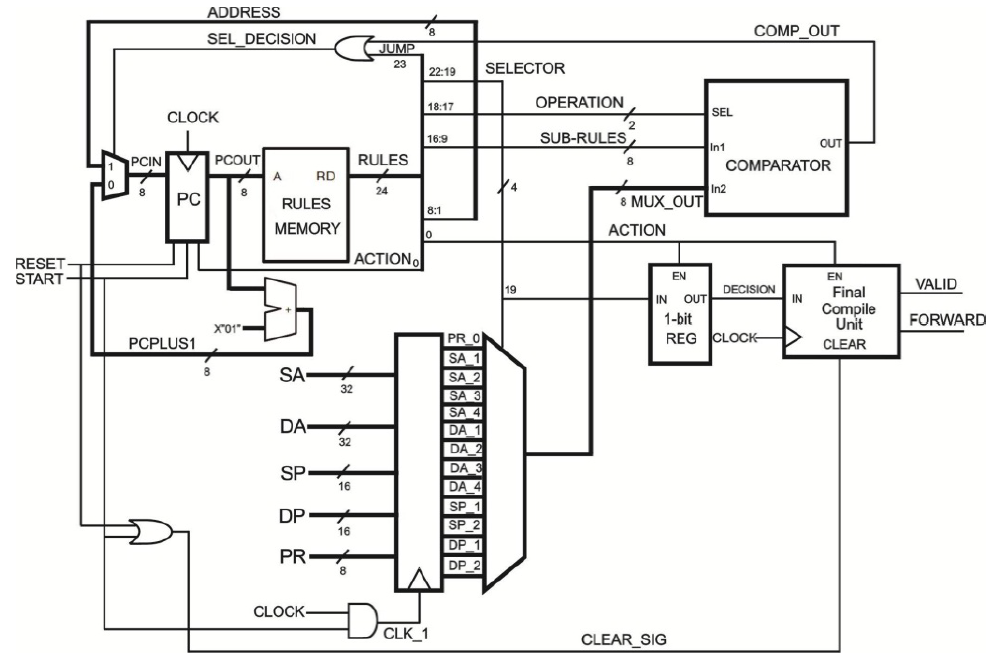
\includegraphics[width=0.8\textwidth]{Images/packetFilterHardware.png}
    \caption[Packet classifier]{Packet classifier \cite{FastRecongifFPGAFirewall}}
    \label{fig:fast-fpga-classifier}
\end{figure}


\newpage

Wasti \cite{Wasti2001HardwareAP} presents several other classification algorithms for both hardware and software packet filters. \textit{'Sequential matching'} provides the most 
trivial solution as it matches each rule to the incoming packet. While simple, this design has scalability issues as more rules get added. Another method proposed in 
\cite{Wasti2001HardwareAP} is by using a \textit{'Grid of tries'} which uses tries (a type of tree datastructure) to help pattern match the packets, but fails to extend to multiple fields. 
Hardware algorithms using \textit{Ternary CAMs} (stores words with 3-valued-digits - namely '0', '1' and '*') and \textit{Bit-parallelism} were also discussed. Both of these 
exploited the parallelised nature of hardware design. One limiting factor with the classification methods cited in \cite{Wasti2001HardwareAP} is their configurability and 
expandability. 



\section{RISC-V processor}
In the world of processor architectures, there are four major families, namely AMD64, x86, ARM and RISC-V. The two former instruction set architectures (ISA) 
are apart of the complex instructions sets (CISC) and are found in the majority of computers. ARM and RISC-V have a reduced instruction set compared to the CISC family and 
subsequently fall under the RISC family and are ideal for low power microprocessors \cite{RV16Embedded}.

RISC-V is an open and royalty free ISA and as a result, a plethora of softcore based custom implementations have been designed \cite{CatalogRISCSoftcore}. 
Consequently, there is an abundance of articles delving into RISC-V from evaluating the ISA \cite{InvestigatingRiscv} to creating multicore architectures
\cite{RiscVMulticore}. A 2019 paper, \cite{CatalogRISCSoftcore} evaluated a variety of different RISC-V softcore processors. RISC-V International have 
also published a list\footnote[1]{See: https://github.com/riscv/riscv-isa-manual/blob/master/marchid.md} of different RISC-V implementations 
that have a unique architecture ID. The majority of these are either written in a HDL for either application specific integrated circuits (ASICs) or FPGAs.
The \textit{NEORV32 RISC-V} softcore processor is written purely in vendor-agnostic VHDL and importantly has a considerable amount of documentation. 

Being a softcore processor, control is given over which modules are implemented. Some basic features of the \textit{NEORV32 RISC-V} include 
UART, SPI, and GPIO interfaces \cite{neorv32Datasheet}. The datasheet, \cite{neorv32Datasheet}, also mentions that it supports a \textit{'Wishbone b4 classic'} 
external bus interface. A Wishbone B4 (or just 'wishbone') interconnection is designed specifically to connect modular pieces of hardware together on a 
SoC into the memory mapped 32bit address space in the processor \cite{WishboneSpec}. This approach has the benefit of not needing to create custom 
instructions for the microprocessor. 


\section{Ethernet MAC}

First introduced in 1983, the IEEE 802.3 standard \cite{IEEE802.3-2012}, more commonly known by the name of 'Ethernet', defines the \textit{'Medium Access Control'} 
(MAC) protocol amongst other things for two or more devices to communicate over a network. This standard is just one part in the layered network 
models such as the OSI model or TCP/IP model, namely the network layer - layer 2. 


A core function of the Ethernet MAC is to attach the required MAC layer headers to the head and tail of the layer 3 payload to create an Ethernet packet. The fields 
in an Ethernet packet can be seen in figure \ref{fig:ieee-mac-headers}. 

\begin{figure}[h]
    \centering
    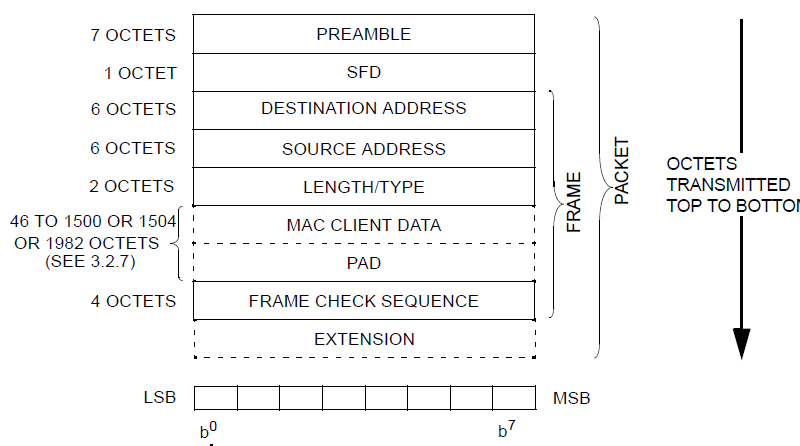
\includegraphics[width=0.65\textwidth]{Images/mac_packet.png}
    \caption[MAC layer headers]{MAC layer headers \cite{IEEE802.3-2012}}
    \label{fig:ieee-mac-headers}
\end{figure}

After the packet has been constructed, the data is forwarded out to the physical (PHY) layer 
least significant bit (LSB) first \cite{IEEE802.3-2012}. Typically, a PHY management chip is used to handle the physical layer channel encoding amongst other things. 
These PHY chips often can be interfaced with the media independent interfaces such as MII, RMII, GMII and RGMII \cite{OptimisedEthernetMAC}. The reduced media 
independent interface (RMII) is one of these standards defined in \cite{IEEE802.3-2012} and consists of a reference clock, 2 bit wide transmit (TX), 2 bit wide 
receive (RX) lines and a few other supplementary signals as defined in the LAN8720A datasheet \cite{LAN8720ADatasheet}.


The MAC layer itself is usually implemented in hardware as it has several advantages over a software implementation. The core reasons behind this are due to parallelised nature of FPGAs and that parts of the MAC can operate independently \cite{reducedEtherentMacFPGA}. One key example is the calculation of the 
frame check sequence (FCS in figure \ref{fig:ieee-mac-headers}). The FCS for Ethernet is a 32bit cyclic redundancy check (CRC) \cite{IEEE802.3-2012} and 
in addition to Etherent, the CRC32 can be found in an extensive amount of applications. As such, research has been conducted into parallelising the calculation. 
Noteably, Mitra and Nayak \cite{ParallelCRC} proposed a low latency parallelised architecture for FPGA design on CRC32. As a result, packets can be assembled 
faster and offload additional processing burden from the CPU. 


Numerous articles \cite{OptimisedEthernetMAC} \cite{EthernetAXI} \cite{EthernetRMII} can be found about Ethernet MACs implemented 
on FPGAs each with a slightly different approach. Fundamentally though, as best highlighted in \cite{OptimisedEthernetMAC}, a simple way of implementing a MAC is by employing a finite state 
machine (FSM) to set the required fields. Another technique found in these articles is the use first-in first-out (FIFO) buffers to cross clock domains. This is a common technique used 
in FPGA design as it allows you to have the packet assembly logic at a much higher clock rate than the output RMII reference clock speed \cite{EthernetAXI}. 

In addition to the papers, there are a plethora of intellectual property (IP) blocks for xMII interfaces in HDL 
which have their own benefits and drawbacks. Some freely available HDL modules for Ethernet MACs can be found in both a complete \footnote[1]{See: https://github.com/yol/ethernet\_mac} \footnote[2]{See: https://github.com/alexforencich/verilog-ethernet/} 
\footnote[3]{See: https://opencores.org/projects/ethernet\_tri\_mode} and incomplete state
\footnote[4]{See: https://github.com/pabennett/ethernet\_mac}.






\section{Web servers and network stacks}

Almost all firewalls need to be configured with a ruleset which can be configured in two common ways, using a command line interface (CLI) 
or by a web-based graphical user interface (GUI). Before a web server can be realised, the network stack (Layers 3, and 4) need to be established since a web server 
operates at the application layer (layer 4). As embedded platforms are resource limited, special precautions need to be taken into consideration when it comes to memory and resource 
usage \cite{OptimCortexLwIP}.

Article \cite{LwIPFPGAFirewall} investigated using the open source lightweight IP (LwIP) network stack as a mechanism for interfacing with the firewall. 
The LwIP library is a popular lightweight TCP/IP stack which has been investigated in a plethora of research papers and projects \cite{ImprovemntOptimLWIP} 
\cite{OptimCortexLwIP}. Often these papers run LwIP on real time operating systems (RTOS) such as FreeRTOS or Zephyr.

FreeRTOS is a leading RTOS for microprocessors and is distributed freely under the MIT license. As an RTOS, it provides an abstraction to the hardware that allows 
for multitasking and brings other OS-Like features to embedded systems. Several ports are available including one for RISC-V. 

FreeRTOS also provide their own TCP/IP network stack called \textit{FreeRTOS-Plus-TCP} which includes a HTTP web server example and is much newer than LwIP.
Consequently, less research can be found apart from existing documentation. The library aims to provide a threadsafe Berkley sockets API and network stack 
supporting multiple protocols such as DHCP, DNS, TCP, and UDP \cite{FreeRTOSTCP}. LwIP is not threadsafe and typically suffers from memory issues as found 
in \cite{OptimCortexLwIP}.





% ***************************************************
% Example of an internal chapter
% ***************************************************
%This is an internal chapter of the thesis.
%If you have a long title, you can supply an abbreviated version to print in the Table of Contents using the optional argument to the \chapter command.
\chapter[Design overview]{Design overview}
\label{chap:methodology}	%CREATE YOUR OWN LABEL.
\pagestyle{headings}

This chapter details the design decisions and steps taken to complete the project. The project itself can be broken down into three main areas: hardware, firmware and software. 


\section{Hardware}
\subsection{FPGA}
Digilent, parented by National Instruments, make a wide range of Xilinx based FPGA development boards and test equipment. In this project, the Digilent Nexys A7-100T FPGA development board (figure \ref{fig:fpga_dev_board}) was used due to it's availability and features including: a Xilinx Artix 7 100T FPGA (part number XC7A100T-1CSG324C), LAN8720A 100MBit/s RMII PHY, micro SD card slot and PMOD (auxiliary outputs) among other IO. 

Xilinx has multiple FPGAs in their 7-series lineup with different target audiences. The Artix-7 family is optimised for low power designs with high logic throughput. The XC7A100T has 101,440 logic cells, 4,860Kbits of Block RAM (BRAM) and 240 DSP blocks \cite{Xilinx7SeriesDatasheet}. There is a varient of the Nexys A7 FPGA board that consists of a XC7A50T FPGA (fewer resources), but ultimately the XC7A100T variant was used due to its larger amount of resources.  

Importantly, there are four ways this FPGA can be configured (essentially \textit{'programmed'}), at each power on cycle using JTAG, nonvolatile SPI flash, microSD card or using a USB stick through the HID interface. These modes are switchable using jumpers, JP1 and JP2, on the board. The JTAG interface is ideal for testing and as such it was used throughout development process, while storing these configurations on a microSD card was used once the design was solidified. 

\begin{figure}[h!]
    \centering
    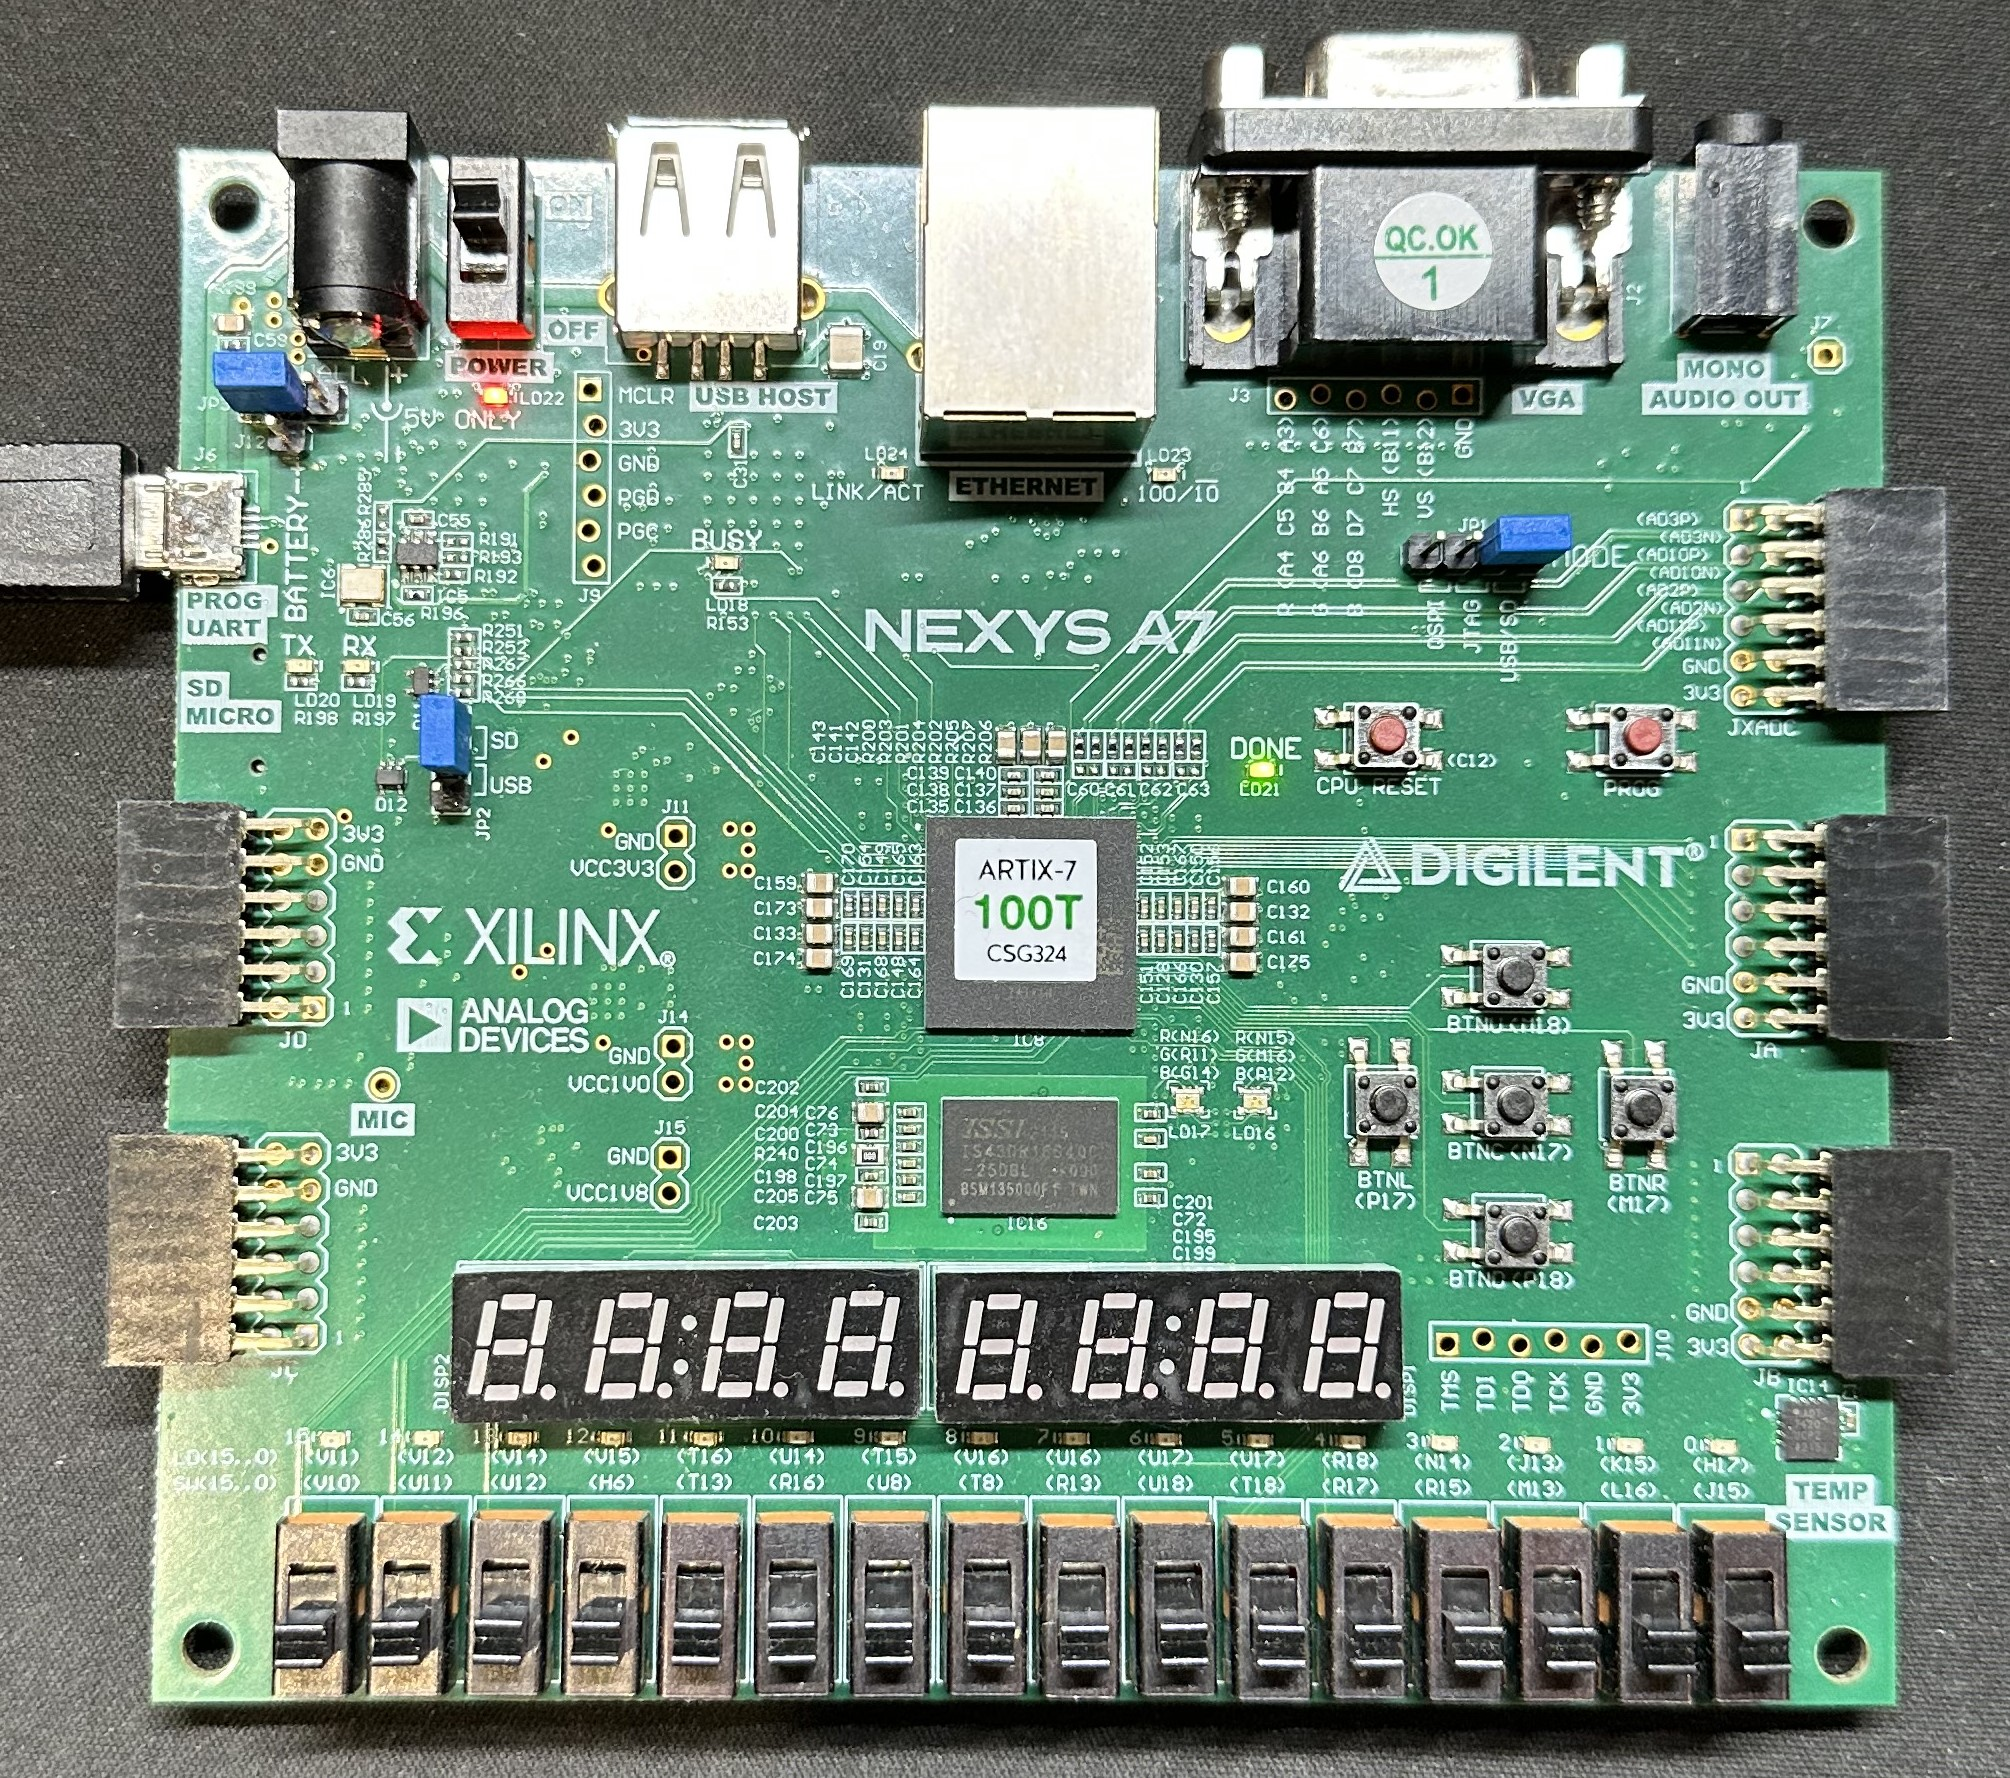
\includegraphics[width=0.65\textwidth]{Images/nexysa7_board.jpg}
    \caption[Digilent Nexys A7 FPGA development board]{Digilent Nexys A7 FPGA development board.}
    \label{fig:fpga_dev_board}
\end{figure}

\newpage






\subsection{MicroSD card}

After the FPGA has been configured using the microSD card, the onboard microcontroller on the Nexys A7 board power cycles the microSD card and relinquishes control of the bus. On power up of the RISC-V softcore processor, it has full control of the card. 

The selected MicroSD card for use in this project is the Patriot LX Series 32GB card, seen in figure \ref{fig:microsd_card}. SD cards, like the patriot card have 2 modes of operation: native SDIO mode and SPI mode. While the native SDIO mode allows for higher speeds, it adds complexity to the design. As the files stored on the SD card are minimal ($< 100KB$), to keep things simple, the microSD card was connected in SPI mode.

\begin{figure}[h]
    \centering
    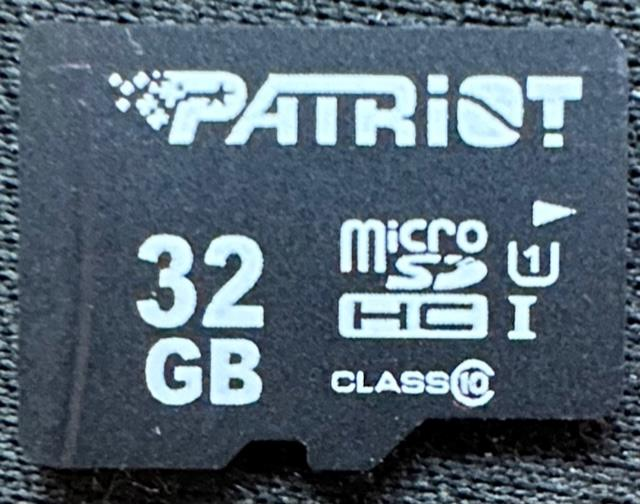
\includegraphics[width=0.2\textwidth]{Images/microsdcard.jpeg}
    \caption[MicroSD card used in project]{MicroSD card used in project.}
    \label{fig:microsd_card}
\end{figure}


The files that were stored on the microSD card include the bitstream file for the FPGA itself and web assets for the webserver. While the bitstream file needed to be at the root directory of the filesystem, the web assets were stored in their own folder structure to help segregate the files.  








 
\subsection{System on Chip}

A benefit to using an FPGA is that full control is given to the overall system design. At the heart of the SoC, a NEORV32 softcore processor\footnote[1]{See: https://github.com/stnolting/neorv32} controls the hardware and runs the higher layers of the network and webserver tasks.

The NEORV32 processor is RISC-V compatible and designed by GitHub user \textit{stnolting} and is highly configurable. In this design, seen in figure \ref{fig:soc_architecture}, the Wishbone, SPI, UART and external interrupts interfaces were enabled and configured. In addition to these, the M extension (Multiplier) was configured to use the DSP blocks to reduce the number of LUTs needed to handle multiplication in the core. 

The Wishbone B4 classic bus is an open source interface that allows for multiple bits of hardware to connect and communicate together. In this project, the bus is 32bits wide and clocked at 80MHz, giving a bandwidth of $32 \times 80 \times 10^6 = 2.56\times 10^9bit/s=2.56Gbit/s$. Due to its relatively high bandwidth, it was used to connect the MAC with the NEORV32 as packets of 1500 bytes would need to be transferred quickly to not bottleneck the 100Mbit Ethernet interface. In addition to this, the MAC had an interrupt line to the NEORV32 processor to notify it when a packet has been recieved and ready for processing in the higher layers. This connects into the XIRQ lines which creates a fast interrupt request by firing a mcause trap event (RISC-V terminology).

Serial Perhipheral Interface (SPI) was used to connect to both the MicroSD card and Packet classifier. These are comparatively low speed and low priority perhipherals and so do not require a high speed interface. UART was connected to the onboard serial to USB converter chip for CLI commands and debugging. 



\begin{figure}[h]
    \centering
    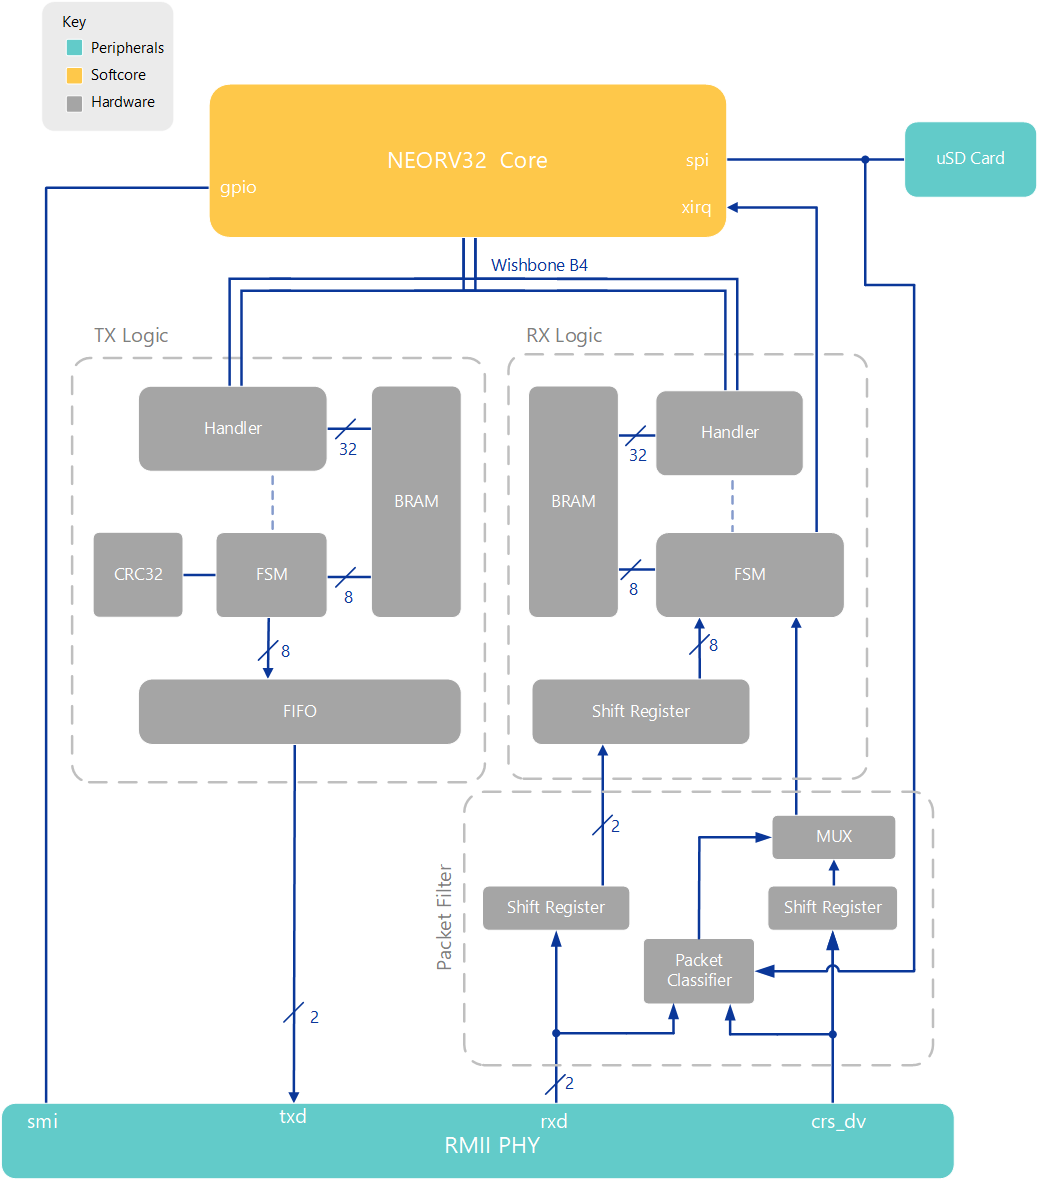
\includegraphics[width=0.85\textwidth]{Images/SoCArchitecture.png}
    \caption[System on Chip high level architecture]{System on Chip high level architecture.}
    \label{fig:soc_architecture}
\end{figure}

\newpage

Since the design is only concerned about incoming filtering, the packet filter was only placed between the RMII PHY and the MAC. By filtering at the RMII interface level, the Ethernet MAC is indifferent to the filter and ultimately doesn't care about it. This allows for a simpler modular design compared to integrating the filter in the MAC hardware. This filter consists of classifier (discussed in section \ref{sec:packet_classifier}) which would determine whether to forward or block an incoming packet.

To do the filtering itself, a shift register can be used to essentially delay the inputs from the RMII PHY until the packet classifier has determined whether to forward or drop the packet. A simple MUX can then be used to either allow the packet to enter the wishbone MAC or to not. 

As the hardware in the MAC only processes the input if crs\_dv is high, we only need to gate the crs\_dv and can always have the rxd lines always attached. However, these should also go through a shift register.

By doing this, it means that we can operate the filter at wirespeed with the only downside is the extra latency that the shift registers bring. The delay that these registers add to the latency can be found to be $T_{latency} = N\times T_{clk}$ where $N$ is the size of the registers. In the design a size of 224 ticks was used. This is because at a minimum, the packet classifier needed to input a maximum of $22 + 24 + 4 = 50$ bytes (22 for MAC headers including preamble, maximum 24 bytes for IP header and 4 bytes for the TCP/UDP headers (only need to check the source and destination port)) need to be processed. While this is enough, a margin of 6 bytes was arbitrarily chosen to allow propagation of other parts of the design to have taken effect. This gave 56 bytes, where each byte takes 4 clock cycles to input into the MAC meaning that we need a register size of $56 \times 4=224$ for the data to propagate to the end of the registers after the packet classifier has determined whether to drop or allow the packet. Importantly this does not effect the speed/bandwidth of the connection. 


It is assumed that any traffic leaving from the device is safe and trusted. In a larger network where there are several devices behind the firewall, it may be desirable to also have a packet filter on the output. 


% amalgamates 








\subsection{Ethernet Media Access Controller}
\label{sec:ethernet_mac}
The advantage of using an FPGA is that custom hardware can be designed for specific tasks. In this design the MAC layer was done in hardware to free up the microprocessor by handling the lower level logic. 

This MAC was implemented as a memory-mapped perhipheral which used the MCU's Wishbone B4 classic interface. This then made it easily accessible over the memory address space of the MCU.  



The hardware can be broken down into two main sections: the transmit logic and receive logic. 

In the receive logic, there are two main functions, one that stores the incoming frame into BRAM and then another to interface the BRAM with the Wishbone interface. On the input side the data is shifted into a 8bit wide shift register - shown in figure \ref{fig:soc_architecture}. While crs\_dv is asserted, after every four clock cycles (modulo four since 2 bits is received at a time) the contents of the shift register is stored into BRAM. After each byte has been added to BRAM, a counter is incremented to store the next byte in the next index. The end of the packet is signified when crs\_dv is deasserted, at which point the payload length is stored for use when the processor receives the frame over the wishbone interface. After the first two bits equals "01" (first 2 bits of the preamble) have been received, a trigger output is asserted so that it can fire a CPU interrupt.

On the wishbone side of the receive logic, only read requests are accepted and processed. A register access returns the payload size of the received frame to help the driver (section \ref{sec:ethernet_mac_driver}) identify how much data it needs to extract from the hardware buffer. When accessing the BRAM memory locations over the Wishbone interface two things are considered. The first is that an offset of eight is needed since the BRAM stores the preamble and SFD which is not wanted by the processor. The second is that the payload is stored in 8bit values whereas the wishbone interface can send 32bits at once. Therefore some conversion between the memory addresses and the memory accesses to BRAM take place. 

\begin{lstlisting}[language=VHDL, caption=Wishbone access logic for Ethernet receive]
if wb_i_stb = '1' and wb_i_addr(31 downto 16) = x"1338" then 
    wb_o_ack <= '1';
    if wb_i_we = '0' then -- Ensure write enable is reset to read.
        if wb_i_addr(15 downto 0) = MAC_DAT_SIZE then -- Payload size
            wb_o_dat <= std_logic_vector(to_unsigned(payloadLen, 32));
        elsif wb_i_addr(15 downto 0) >= x"0008" and wb_i_addr(15 downto 0) <= x"05F8" then -- BRAM access
            virtAddr := to_integer((unsigned(wb_i_addr(15 downto 0)) - 8));
            wb_o_dat <= FRAME_BUFFER(virtAddr) &  FRAME_BUFFER(1 + virtAddr) & FRAME_BUFFER(2 + virtAddr) & FRAME_BUFFER(3 + virtAddr);
        end if;
    end if;
else
    wb_o_ack <= '0';
end if;
\end{lstlisting}

By splitting the address over 2 if conditions, the amount of resources can be greatly reduced as the nested if conditions only need to compare 16bits instead of 32bits each time. Another important design decision is that this version of the Ethernet MAC does not validate the FCS after receiving a packet, instead it assumes it's a valid packet. 


The transmit logic is broken down into three parts: Wishbone handler, main FSM and RMII conversion. The process of creating and sending an Ethernet frame starts with the processor sending data over the Wishbone interface. Like the receive logic, there are two types of commands that can be sent over the Wishbone interface, one that controls the logic, the other that stores payload data into BRAM. There are three configuration commands, one to initialise the hardware and FSM, another to start the transmission of data (used after all data has been transferred into BRAM) and one to set the payload length of the packet. The other register addresses allow the processor to store the payload in the frame buffer (BRAM). See figure \ref{fig:bram_frame_format} for the format of data in BRAM. The preamble, SFD and FCS are left out as these are appended in hardware. To be accurate, this is a quasi-MAC as the MAC addresses and type fields in the header (expanded view of payload in figure \ref{fig:bram_frame_format}) are populated in software. 

\begin{figure}[h!]
    \centering
    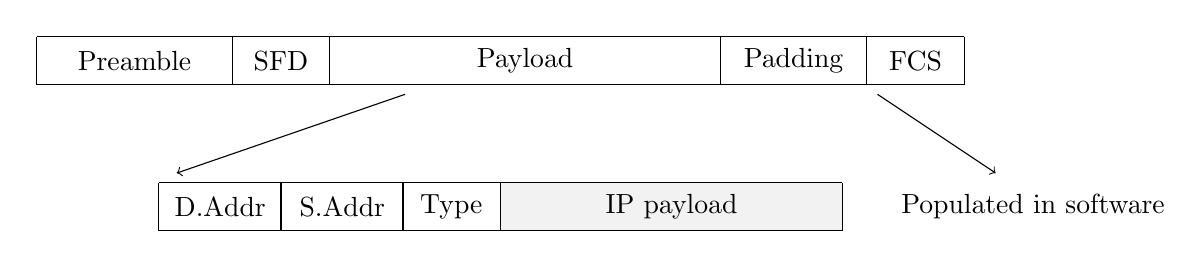
\begin{tikzpicture}

        % First bytefield
        \node (a) {
            \begin{bytefield}{8}
                \bitbox{8}{Preamble} & \bitbox{4}{SFD} & \bitbox{16}{Payload} & \bitbox{6}{Padding} & \bitbox{4}{FCS} 
            \end{bytefield}
        };

        % Expanded Payload
        \node[below=1cm of a.south] (b) {
            \begin{bytefield}{16}
                \bitbox{5}{D.Addr} & \bitbox{5}{S.Addr} & \bitbox{4}{Type} & \bitbox{14}[bgcolor=lightergray]{IP payload}
            \end{bytefield}
        };

        \node[right=0.5cm of b.east, anchor=west] {Populated in software};

        % Connection lines
        % Arrow from the left side of Payload to Field 1
        \draw[->] ([xshift=4.8cm]a.south west) -- ([xshift=0.35cm]b.north west);

        % Arrow from the right side of Payload to Field 3
        \draw[->] ([xshift=10.8cm]a.south west) -- ([xshift=10.75cm]b.north west);

    \end{tikzpicture}
    \caption{Format of frame in BRAM}
    \label{fig:bram_frame_format}
\end{figure}


Once a payload has been stored in the frame buffer, the main FSM takes control and at this point the CPU is free to do anything else. Since the FCS is calculated in hardware, the FSM resets the FCS hardware and begins to send the bytes to both the FCS hardware (to calculate the CRC32) and to a FIFO buffer. Once the payload has been transmitted to the FIFO, the resulting CRC32 FCS is sent out to the FIFO without missing a clock cycle. 

A FIFO buffer is used to cross the domains since the RMII interface is 50MHz at 2bits wide, whereas the bytes are stored as 8bit vectors in the frame buffer. This also allows the FSM to have a higher clock speed as well. The current implementation of the FSM uses a 80MHz clock signal, consequently the equivalent bit rate is 6/4 times larger than the output needed to the RMII interface. The FIFO used in this design, figure \ref{fig:fifo_diagram}, is slightly modified so that the read clock is one quarter the 50MHz output frequency since the FIFO itself returns 8 bits at a time. An FSM operating at 50MHz then sends each 2bit nibble out to the RMII PHY at a time in a circular fashion. The tx\_en line is asserted while the FIFO is non-empty.


\begin{figure}[h!]
    \centering
    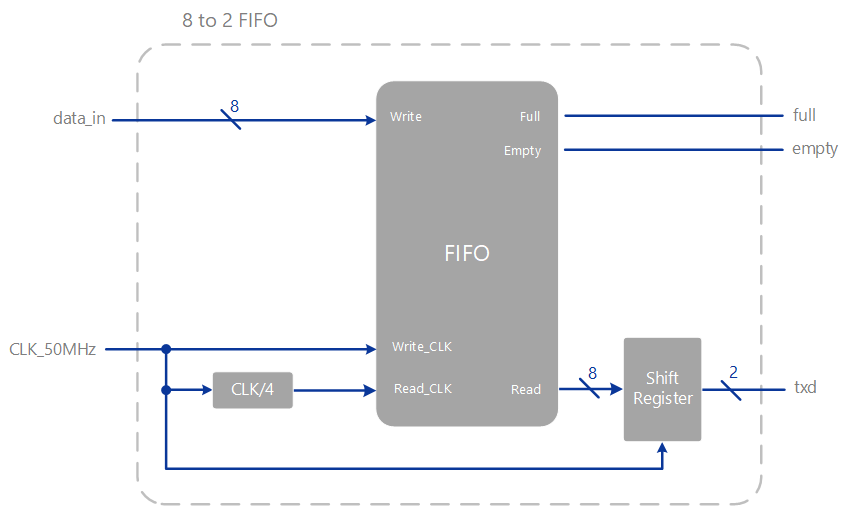
\includegraphics[width=0.75\textwidth]{Images/EthFIFO.png}
    \caption[8bit to 2bit FIFO used for RMII output]{8bit to 2bit FIFO used for RMII output.}
    \label{fig:fifo_diagram}
\end{figure}




The documentation for the NEORV32 states that all memory accesses that do not target specific processor-internal address regions (see appendix \ref{app:mem_address}) get forwarded to the external interfaces, such as the Wishbone interface. As such, there is a large block of unused memory between the IMEM and DMEM regions. The memory mapping, figure \ref{fig:memory_layout}, used in this design ranges from 0x13370000 to 0x133805F8.


% \begin{tikzpicture}[remember picture,overlay]
%     % Define coordinates for shading
%     \coordinate (top-left) at (3.95, -0.05);  % Adjust as necessary
%     \coordinate (bottom-right) at (10, -2.5); % Adjust as necessary
    
%     % Draw shading
%     \fill[gray!30] (top-left) rectangle (bottom-right); % Change gray!30 to your desired shading color and intensity
% \end{tikzpicture}

\begin{figure}[h!]
    \begin{center}
    
\begin{bytefield}{24}
% \memsection{ffff ffff}{0040 0000}{5}{Processor memory}\\
\memsection{1338 05F8}{1338 0008}{5}{RX PAYLOAD}\\
\memsection{1338 0007}{1338 0004}{2}{RX SIZE}\\
\memsectioncolour{1338 0003}{1337 6411}{3}{Unused}\\
\memsection{1337 6410}{1337 1004}{4}{TX PAYLOAD}\\
\memsection{1337 1003}{1337 1000}{2}{TX SIZE}\\
\memsection{1337 0003}{1337 0000}{2}{TX CONFIG}\\
% \memsection{1336 ffff}{0000 0000}{5}{Processor memory}
\end{bytefield}
\caption{Memory Address Layout}
\label{fig:memory_layout}
\end{center}
\end{figure}

This mapping is required for developing the driver (section \ref{sec:ethernet_mac_driver}) to access the correct registers.









\subsection{Packet Classifier}
\label{sec:packet_classifier}
To further save MCU resources, the packet classification was done in hardware. Not only did this reduce the load on the MCU itself - giving it more time to do other things - it allowed the interface to run at \textit{'wirespeed'}. That is, at the full speed of the interface - 100Mbit/s. 

This was possible by having the rulset been evaluated in parallel as the data is coming into the firewall. This method however is not suitable for large rulesets as the fan-in and fan-out limit the maximum number of parallel comparisons. For every new rule, the number of gates grows exponentially. Hence a design decision of a maximum ruleset of size 8 was chosen. 

The way this classifier was designed was to be a \textit{'default-block'} where all connections were blocked except for the ones specifically whitelisted in the ruleset. The specific rules had a few options, namely the source IP address, destination IP address, source port, destination port and protocol could be configured. In addition to these, each field had a wildcard operator which allowed all values for that specific option to be classified. 


The design of the packet classifier hardware, figure \ref{fig:packet_classifier_architecture} stores the firewall rules in block memory. The rules are stored in BRAM as an array of 112 bits with the format shown in figure \ref{fig:pc_rule_format}.


\begin{figure}[h!]
    \centering

    \begin{bytefield}{8}
        \bitbox{6}{$Wildcard$} & \bitbox{5}{$IP_{Dest}$} & \bitbox{5}{$IP_{Src}$} & \bitbox{6}{$Port_{Dest}$} & \bitbox{6}{$Port_{Src}$} & \bitbox{6}{$Protocol$} 
    \end{bytefield}
    
    \caption{Format of rules stored in BRAM}
    \label{fig:pc_rule_format}
\end{figure}


The wildcard attribute signifies whether to allow all possible combinations (in other words, disregard) for the positional attribute where the most significant bit refers to the $IP_{Dest}$ and the least significant bit refers to the $Protocol$.

A FSM then records the position of the incoming and configures the multiplexers on the BRAM to output the current property to the comparators where they compare with the shift register which contains the current field being classified. On a successful match, a bit is left set in the result register, otherwise clear if no match. Importantly, the bits only get set on the first iteration of the classification. 

After passing through all the fields, if there is any bit set in the results register, it indicates that a rule matched and that a packet should be forwarded. 


\begin{figure}[h!]
    \centering
    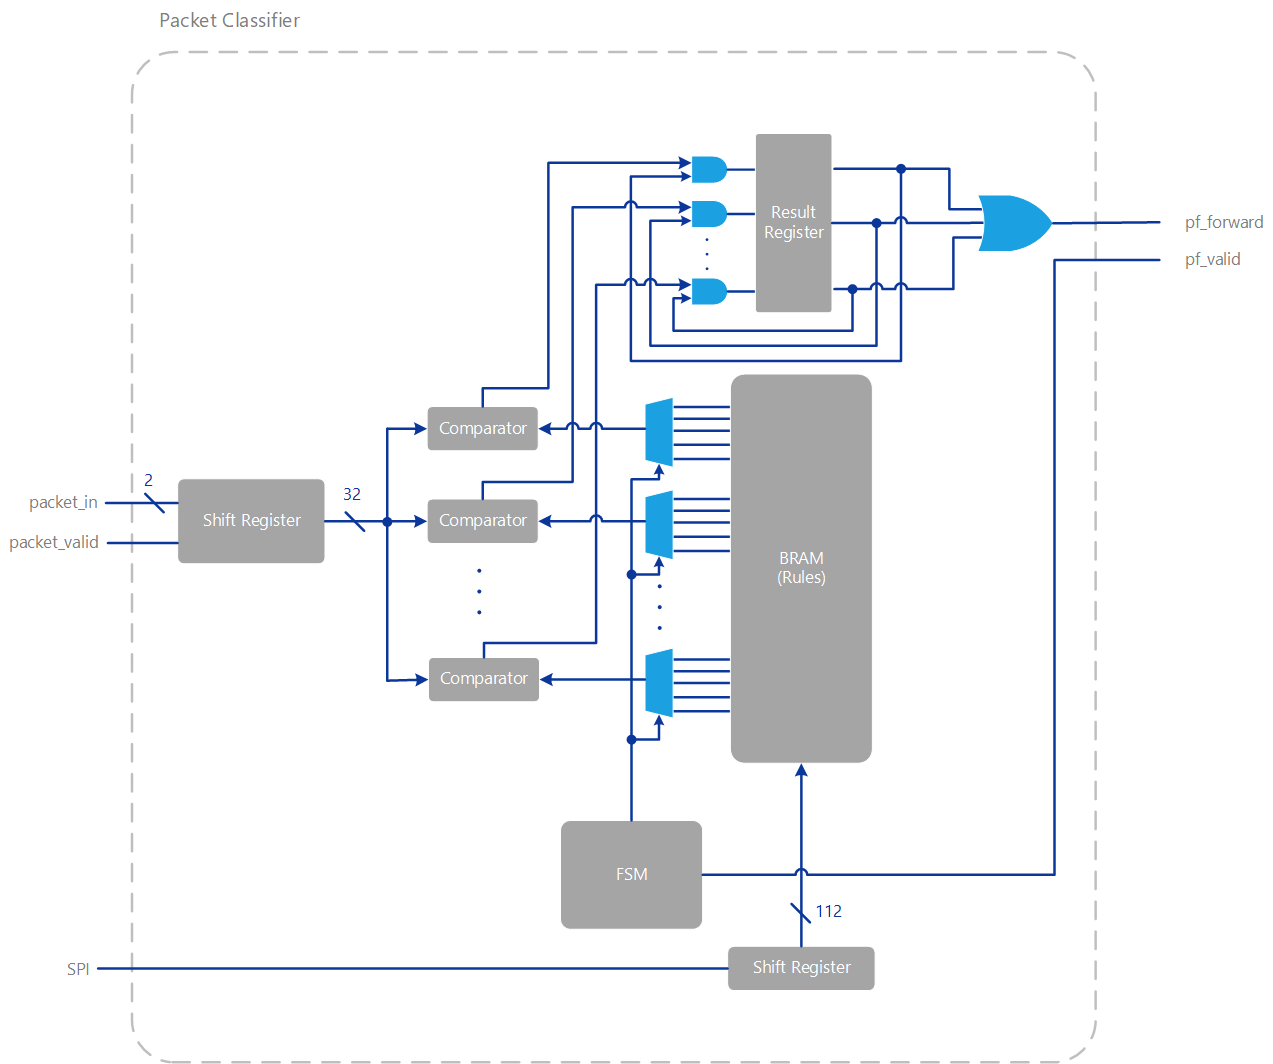
\includegraphics[width=1\textwidth]{Images/PacketFilterArchitecture.png}
    \caption[Packet classifier architecture]{Packet classifier architecture. Clock signals have been omitted.}
    \label{fig:packet_classifier_architecture}
\end{figure}

This reduces the required resources as only 1 set of comparators are needed, which is important as for each rule that exists, another comparator is needed. In this design, there are a total of 8 comparators, 8 multiplexers and the results register is 8bits wide. 

A more resource efficient design is possible at the cost of latency. This is one of the critiques of the design mentioned in \cite{FastRecongifFPGAFirewall} as multiple clock cycles would be needed to classify the headers. In theory the clock speed could be faster than Ethernet frequency and as only two bits from the RMII interface are processed at a time, it could be a viable alternative, however this may likely fall apart when higher speeds are required. 


Several options exist for configuring the ruleset in the packet classifier such as: Wishbone, I2C, UART, SPI or a completely custom solution. For simplicity, SPI was used in configuring the packet filter. Importantly, data would only flow in one direction, from the microcontroller to the classifier and not the other way round. This means that the microcontroller needs to keep the state of the rules inside the packet filter and needs to resend the rules to be sure of the configuration. This is not an issue as the rules need to be stored in flash on the microSD card to keep settings between power cycles. The format, figure \ref{fig:spi_message_format} that the SPI hardware expects is similar to how it's stored in BRAM to make it quick and easy to transfer.

\begin{figure}[h!]
    \centering

    \begin{bytefield}{8}
        \bitbox{6}{$Index$} & \bitbox{6}{$Wildcard$} & \bitbox{5}{$IP_{Dest}$} & \bitbox{5}{$IP_{Src}$} & \bitbox{6}{$Port_{Dest}$} & \bitbox{6}{$Port_{Src}$} & \bitbox{6}{$Protocol$} 
    \end{bytefield}
    
    \caption{Format of SPI messages}
    \label{fig:spi_message_format}
\end{figure}



Notably, the data is received into a shift register and after all bits have been received the BRAM is updated at the corresponding index in a single clock cycle.








\section{Firmware}
\subsection{Ethernet drivers}
\label{sec:ethernet_mac_driver}

Since the Ethernet hardware was custom, drivers were needed to interface with the hardware in software. There were two types of commands that were needed, first the RMII serial managment interface (SMI) and secondly the MAC drivers - the drivers that would handle the data.  The SMI interface is used to control the mode of operation of the PHY chip including the speed, Auto-MDIX, duplex settings. The LAN8720A datasheet, (\cite{LAN8720ADatasheet}) provided some details (seen in figure \ref{fig:smi_packet_structure}) into how the protocol operated. The datasheet also outlined that a maximum frequency of 2.5MHz, but no lower bound. As such the interface was \textit{'bitbanged'} with GPIO pins to reduce complexity. The maximum switching frequency of the NEORV32's GPIO was measured to be $\approx 1$MHz, thus no additional delays were needed in the code and that the GPIO pin could be toggled at the fasted speed possible. 


\begin{figure}[h!]
    \centering
    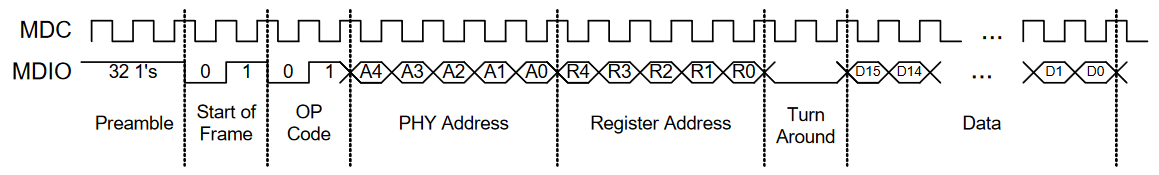
\includegraphics[width=0.75\textwidth]{Images/SMIWriteStructure.png}
    \caption[SMI Write message structure]{SMI Write message structure. \cite{LAN8720ADatasheet}}
    \label{fig:smi_packet_structure}
\end{figure}

On power up the RMII interface would be set to full duplex, 100Mbps and auto-negotiate in accordance to the LAN8720A datasheet. 10Mbit and half duplex modes were excluded from the design as further hardware design would be required.  


As the Ethernet hardware used the Wishbone interface, the register locations were mapped into the processors address space. Accessing these registers is analogous to accessing any other variable in memory, using pointers to the memory address. As an example, to access memory location \codebg{0x12345678} the following C code can be used \codebg{*(volatile uint32_t *) 0x12345678}


To simplify the design and improve readability, a range of macros was setup, such example of macros can be seen below. 

\begin{lstlisting}[language=C, caption=Python example]
#define ETH_MAC_TX_BASE 0x13371000
#define ETH_MAC_CMD_BASE 0x13370000

#define ETH_MAC_CMD  (*(volatile uint32_t *)ETH_MAC_CMD_BASE)
#define ETH_MAC_TX ((EthMacTx *) ETH_MAC_TX_BASE)

typedef struct __attribute__((__packed__))  {
    volatile uint32_t SIZE;
    volatile uint32_t DATA[375]; // 1500 / 4 = 375.
} EthMacTx;
\end{lstlisting}

This allowed for the connected wishbone Ethernet to be accessed like any other register in the embedded system. 


There are three fundamental functions that the driver itself must fulfill, initialisation, send data and receive data. The intialisation resets the Ethernet MAC and resets the interrupt registers. 

The send method is also trivial, but importantly it takes in two parameters, the first is an array of data to send and the second is the amount or length of the data. Like with the SMI interface, these instructions and data transfers were actioned without any delays as the hardware was capable of handling the native speed of the processor. After the data had been transferred, the hardware is instructed to send out the packet. There is no need to provide the FCS as this is calculated on the fly in hardware. 

Similarly, a receive method was created that took in a buffer to store the bytes into as it transfers the data into memory from the registers. Both the transmit and receive functions handled the data translation from 32bit values over the wishbone interface to 8bit bytes in software. In addition to this, as the Ethernet hardware used external interrupts to signal to the processor that there is an Ethernet packet ready for processing. This would use direct task notifications to signal to other functions in the code to call the receive method. 


\subsection{SD card drivers}
\label{sec:microsd_drivers}
To use a micro SD card, drivers must be created so that the card can be initialised, written to and read from. More preciesly, in accordance to the  documentation for the FreeRTOS-Plus-FAT file system, the driver had to implement a function that reads sectors from the media and one that rights sectors to the media. 

Unlike the Ethernet MAC, initialising a MicroSD card isn't as trivial and requires multiple steps. A guide online for AVRs\footnote[1]{See: http://www.rjhcoding.com/avrc-sd-interface-1.php} was followed and the code was ported to the NEORV32 system. In a nutshell, the SPI interface was initalised with a clock divisor of 1 and a prescalar of 3, several commands were sent and recieved from the SD card and then it was put into IDLE mode after increasing the speed of the SPI interface to have no clock divisor and a prescalar of 1.

Similarly, the same guide was followed to implement the read and write sector functions. Importantly, these functions would read and write a whole block at a time. On a microSD card, a block is considered to be 512 bytes. 


In addition to these, a simple function to determine if a SD card is present in the slot was also implemented to warn the user if data was attempted to be written to or read from without a physical card in the slot. 





\subsection{Packet classifier drivers}
\label{sec:packet_filter_driver}
An initialisation function was created to enable and configure the SPI interface on the microprocessor for mode 0, and with no clock diviser and a prescalar of 1. The SPI hardware for the classifier can handle speeds in excess of 80Mhz (seen in section \ref{sec:timing_constraints}), hence there was no need to slow down the clock. Moreover, calling this initialise function is only required if the microSD card intialise function has not been called. 

A single function was created that takes in all the attributes needed in the packet filter and that sends these out in the correct order and format to the hardware. 








\section{Software}

\subsection{Real Time Operating System}
In addition to simplifying the software, an RTOS was used to allow the use of network TCP stacks and handle multiple concurrent connections at a time. FreeRTOS version V10.4.4 was used due to its familirity and compatability with the NEORV32 MCU. FreeRTOS also had integration with their own filesystem (section \ref{sec:freertos_filesystem}) and TCP/IP stack (section \ref{sec:freertos_tcpip_stack}).

\subsection{Filesystem}
\label{sec:freertos_filesystem}
The FreeRTOS-Plus-FAT filesystem library was used to allow the system to read and write files (such as web assets) to a microSD card. The library is managed by FreeRTOS and is DOS compatible which allows FAT32 formatted drives to work. Other popular filesystem modules such as FatFS\footnote[1]{http://elm-chan.org/fsw/ff/00index\_e.html} and LittleFS \footnote[2]{https://github.com/littlefs-project/littlefs} were also considered, but did not have the same level of integration and active support as the FreeRTOS option. 

The library then uses the microSD card drivers (section \ref{sec:microsd_drivers}) to access the disk. 


\subsection{Network Stack}
\label{sec:freertos_tcpip_stack}

Two main options for the network stack were available, LwIP and FreeRTOS-Plus-TCP. The main concern with LwIP was that it was not threadsafe and had memory issues. In addition to this, as FreeRTOS was chosen as the RTOS, their own TCP stack had tighter integration. The stack provides a Berkeley sockets API which is the same used in full-blown operating systems such as Linux. It also includes support for ARP, DHCP, DNS and ICMP protocols, which were used throughout this project. 

Like with the filesystem library, the stack needed to be ported to the NEORV32 processor and importantly the custom Etherent hardware. In addition to the transmit, receive and initalisation methods, functions to return random numbers were needed. These are for the TCP sequence numbers and are required to truely random for security. As such, the hardware based true random number generator in the NEORV32 core was used. 


\subsection{Webserver}
A simple HTTP webserver running on top of a TCP server was used to serve the webpages for the project. FreeRTOS give an example of how to setup a TCP and HTTP server that uses the FAT filesystem to get the content such as the html, css and javascript files. 

... TALK ABOUT WHAT TYPE OF FILES ARE BEEN SERVED, VUE, PLAIN HTML ETC...


\subsubsection{API server}
A subset of the webserver is the API server itself. To make the design simpler, an API was created so that the interface to set and get the firewall rules was independant of the web content. The way the software distinguishes between requests to load a webpage and the API server itself is by inspecting both the route/URL (pcUrlData) and the method type (GET, POST, PUT).

For setting the firewall rules, a POST request to the \textit{'/api/firewall'} endpoint can be made. The body of the request would contain the rule in the following format

\[
payload=Index | Wildcard | IP_{Dest} |  IP_{Src}  | Port_{Dest} |  Port_{Src} | Protocol
\]

Where $|$ is the concatination operator and all fields are in hexadecimal. As an example, to insert a rule at index 0, and with a wildcard operator for all items with a destination IP of 10.20.1.120, source IP of 10.0.0.159, source and destination port of 80 and a protocol of TCP, the following body would need to be sent to the API: \codebg{payload=003F0A1401780A00009F0050005006}. The API server then takes the necessary action and applies the rule to the packet filter by calling the methods in the packet filter driver (section \ref{sec:packet_filter_driver}).



\subsection{Command line interface}

To aid with debugging the FreeRTOS-Plus-CLI framework was used. This would easily allow certain actions to be executed on demand without the need to reflash or reset the device each time. Such examples include configuring the PHY, ethernet MAC, sending ICMP packets and filesystem related commands. In additon, the firewall rules can be set from the CLI in the event that the firewall blocks HTTP connections. 



% ***************************************************
% Example of an internal chapter
% ***************************************************
%This is an internal chapter of the thesis.
%If you have a long title, you can supply an abbreviated version to print in the Table of Contents using the optional argument to the \chapter command.
\chapter[Results]{Results}
\label{Chap:label}	%CREATE YOUR OWN LABEL.
\pagestyle{headings}


To ensure that the firewall was performing properly, a few tests were conducted. In this chapter, the testing results for the performance and the resource utilisation among other features are discussed. 

\section{Modifications}
The design was changed from the 2 ethernet interfaces to a design with just a single ethernet interface. 

\section{Performance}

Talk about wishbone bus speed. 
Initial tests were also conducted at 100MHz, but due to timing issues, it was reverted to 50MHz.


To test the speed of the packet classifier, a Agilent MSO6054A MSO was used (4GSa/s). A pin was set to the output of the crs\_dv of the PHY and the crs\_dv after the packet filter. The time between the rising and falling edge of the output will be the delay added by the packet filter. 


As the shift register in the hardware has a length of 224 bits, at a clock frequency of 50Mhz, the added latency is $224 \times \frac{1}{50\times 10^6} = 4.48 \times 10^{-6} = 4.48uS$. 


\begin{figure}[h!]
    \centering
    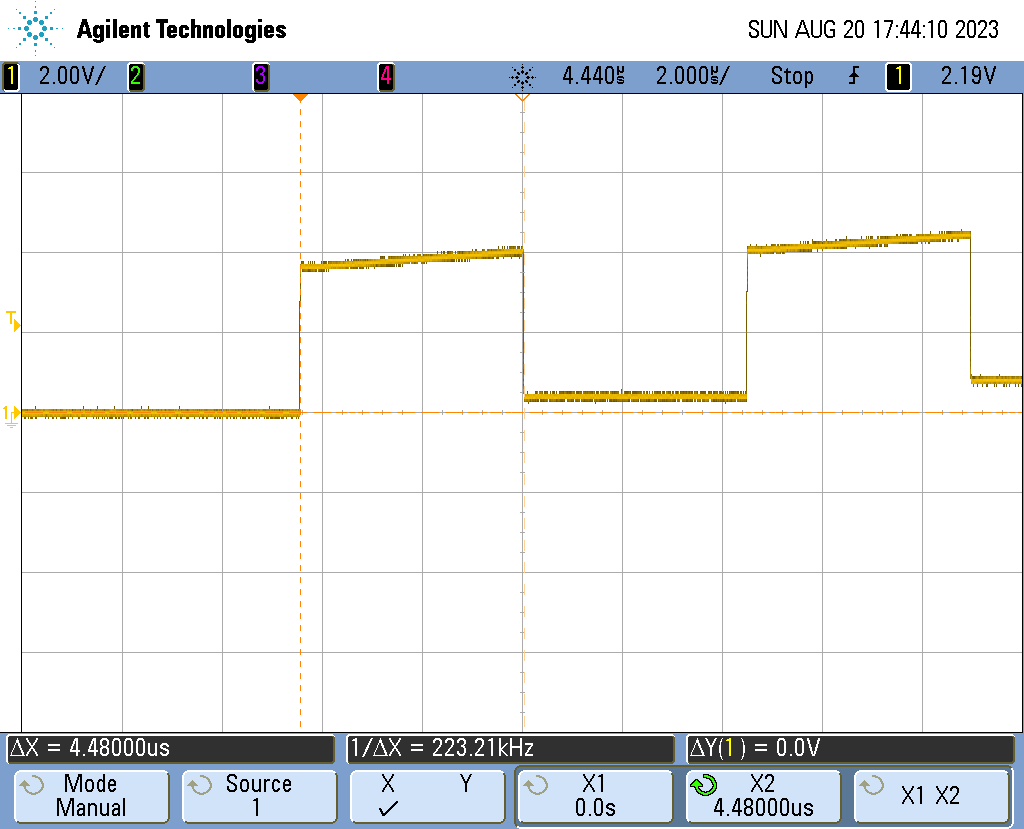
\includegraphics[width=0.75\textwidth]{Images/scope_4.png}
    \caption[Added latency by packet filter waveform]{Added latency by packet filter waveform.}
    \label{fig:packet_classifier_architecture}
\end{figure}

There is two pulses in this graph. This is due to when the crs\_dv line gets disasserted at the end of the packet. From this the time taken to receive the packet can be found to be 8.94uS. This is just an observation and is proportional to the packet size.



The same setup was used to test the preexisting solution, except this time GPIO pins were set high and low. It is assumed that the latency of setting the pin high cancels out with the latency of setting the pin low. 

\subsection{Limitations}
\subsubsection{PMOD Interface}

There are 5 PMOD connectors on the development board. Initally, one of these would be used for a second Ethernet PHY, but due to bandwidth limitations of the interface, the design had to be altered. The recommended bandwidth of these ports are 25MHz while the Ethernet RMII PHY would have been using 50Mhz signals over the interface. As such, signal integrity issues arose (see figure \ref{fig:eye_diagram}) and restricted the use to just one interface - the onboard PHY. A new development board with two PHYs would be needed.

\begin{figure}[h]
    \centering
    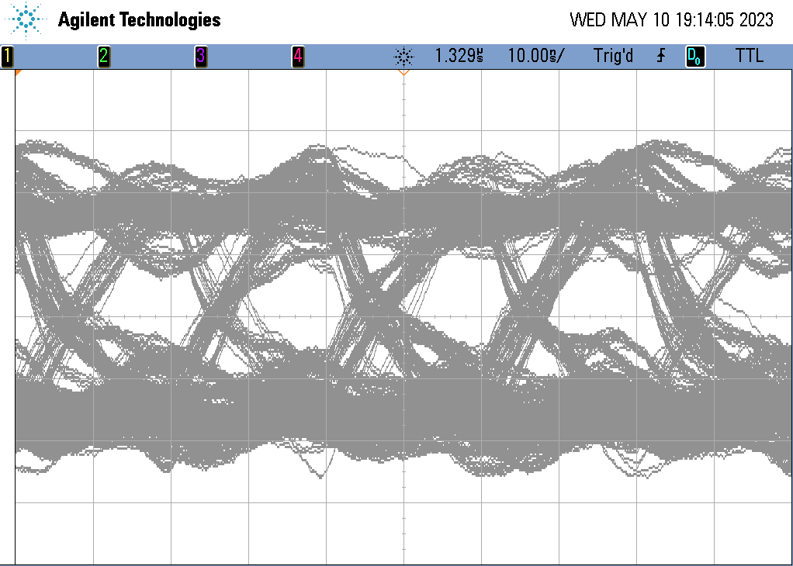
\includegraphics[width=0.65\textwidth]{Images/EyeDiagramTX.png}
    \caption[Eye diagram of TXD through PMOD interface]{Eye diagram of TXD through PMOD interface.}
    \label{fig:eye_diagram}
\end{figure}


\subsection{Testing setup}

\subsection{Results}



\section{Ultilisation}

The design can be broken down into several parts including the NeoRV32 processor itself, Ethernet and packet filtering hardware.

\begin{figure}[h]
    \centering
    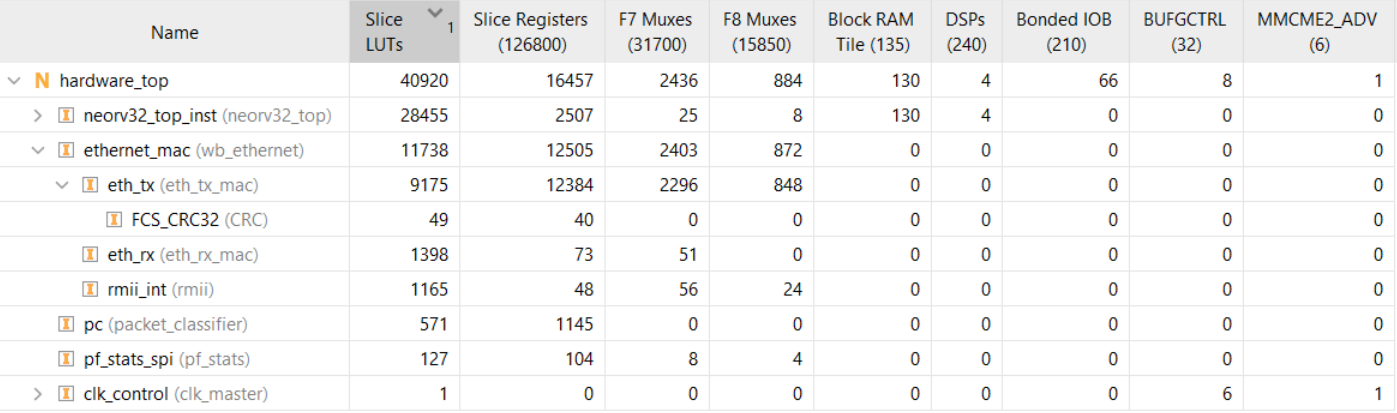
\includegraphics[width=0.85\textwidth]{Images/FPGAUtilisationResources.png}
    \caption[Summary of the resource utilisation on XC7A100T FPGA]{Summary of the resource utilisation on XC7A100T FPGA.}
    \label{fig:eye_diagram}
\end{figure}

The total number of resoruces on the FPGA are as follows: 63,400 LUTs, 126,800 flip flops, 135 BRAM tiles, 240 DSPs and 6 MMCMs.

LUT6 and LUT5 primatives were used the most in the design and by far the FDRE flip flop was the most used flip flop type. 2436 MUXF7s were also used. RAMD64E was also used in the design. The report from vivado can be found in appendix \ref{app:res_usage}.

\subsection{NeoRV32 processor}

The NeoRV32 SoC was configured to use the SPI, UART, GPIO, external interupts (XIRQ), true random number generator and importantly the wishbone B4 classic interface. The DSP48 blocks were used by the SoC to handle the multiply operations as this would free up LUTs and compute the result faster. 

The IMEM and DMEM sizes were chosen to consume as much of the remaining BRAM blocks left as possible. IMEM, the program storage was configured to 256KB while the DMEM, effectively the RAM, was configured to take the remaining amount left and set to 168KB in size. 

After synthesis of the design at 50Mhz, it was deemed that there was some headroom in the critical path delays. Hence the design was updated to 80MHz. This however does not affect the resource utilisation except for taking up some extra clock buffers. A single MMCM was still used to add the additional 80MHz output. 

The NeoRV32 itself took 28455 slice LUTs, 2507 Slice registers, 130 Block RAM tiles and 4 DSPs. 


\subsection{Ethernet hardware}
Comparatively, the Ethernet hardware took 11738 Slice LUTs and 12505 Slice registers, most of which is consumed by the transmit logic. This is largely due to the required buffers when storing (to construct) and sending out the frame. 

\subsection{Packet filter}
The packet classifier took a total of 571 Slice LUTs and 1145 Slice registers. This is lower than expected and indicates that the design could easily be increased to consolidate more rules. However, the fanout of the design will need to be considered due to the nature of the implementation. 





\section{Timing constraints}
\label{sec:timing_constraints}





Testing with WIZ5500 Pico, avg udp rtt was 1.88ms from 1000 tests with a payload of 7 bytes.
Testing with WIZ5500 Pico, avg udp rtt was 2.07ms from 1000 tests with a payload of 256 bytes.

Testing with FPGA board, avg udp rtt was 1.45ms from 1000 tests with a payload of 7 bytes.
Testing with FPGA board, avg udp rtt was 1.72ms from 1000 tests with a payload of 256 bytes.

observations, the WIZ5500 chip was getting excessively hot..

Maybe do a power and thermal camera comparison.


A thermal camera was used to record the temperatures periodically. At an ambient room temperature of $24.8\degree C$ throughout the test, after 5mins the WIZ5500 ethernet chip heated to $58.0\degree C$ and RP2040 was at $46.6\degree C$. While the FPGA was at $38.0 \degree C$. This is a bit of an unfair comparison as the physical size of the FPGA is much larger than the WIZ5500. After two hours of constant UDP ping requests to both devices, figure \ref{fig:thermal_2hr} shows the FPGA board and WIZ5500 board's temperature gradient. The FPGA plateaued to a maximum of $40.4 \degree C$ while the WIZ5500 was $1.c \degree C$ cooler at, $56.8 \degree C$. This could be due to accuracy of the measurements, in addition to not getting aiming the thermal camera in the hottest part. The RP2040 chip however was measured to be $53.2 \degree C$. Some additional thermal images can be found in the appendix.


\begin{figure}[h]
    \centering
    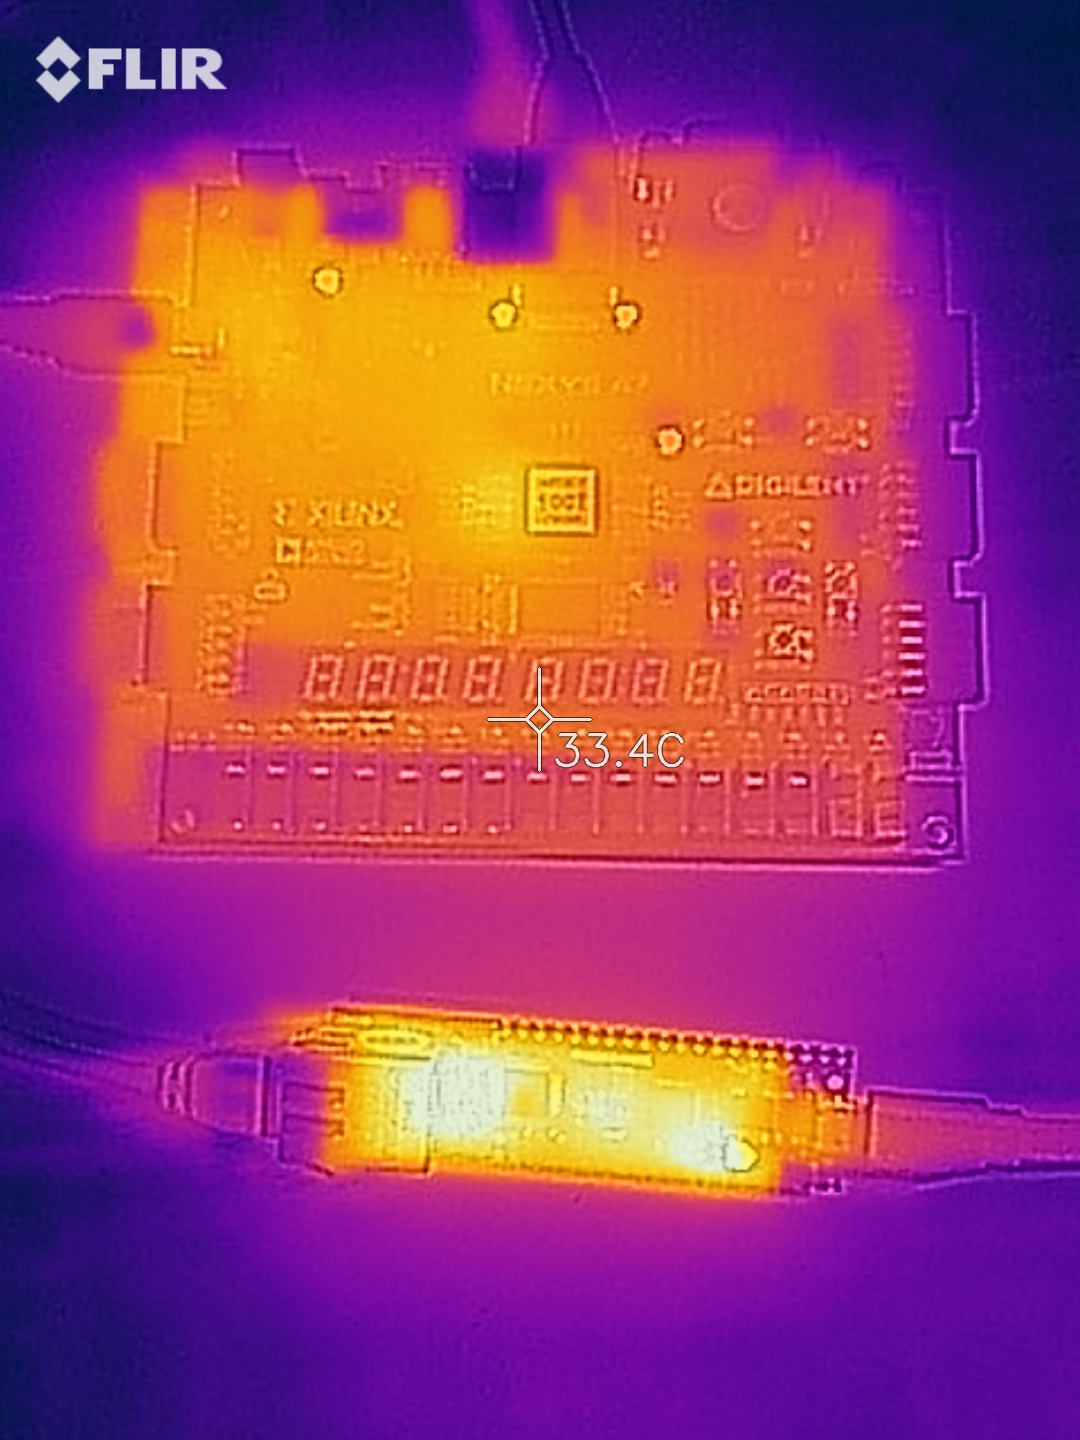
\includegraphics[width=0.5\textwidth]{Images/flir_2hs.jpg}
    \caption[Thermal image of FPGA board and WIZ5500 after two hours]{Thermal image of FPGA board and WIZ5500 after two hours.}
    \label{fig:thermal_2hr}
\end{figure}


\section{Power analysis}

As the voltage would remain constant between devices (all powered over USB), only the current was measured. These results however should be taken with caution as they do not account for regulator inefficiencies and do not give a true current reading of the device, rather just an indication. 


The device for testing the current was the Nordic Semiconductor Power Profiler Kit 2 which can record at up to 100kSa/s. For the tests in this report, only a sampling rate of 10kSa/s was used as it produces less noisy results. 

As a baseline, the Nexys A7 board draws 200mA with no design applied and is due to all the additional components on the board. With the design loaded up but without the processor flashed, the board took 284.4mA. After flashing the board, the idle current reached an average of 301.84mA.

A series of tests were then done and the currents were measured. By pinging the device every 50ms, the average current consumption was 300.72mA. Interestingly, the current consumption was cyclic similar to what is shown in figure \ref{fig:ppk_icmp_ping}. A UDP ping test was conducted and had an average current draw of 301.13mA. In both the ICMP and UDP pings, the current consumption was of similar style where the variance of the current was about 10mA. 


If the packets are now blocked by the filter, more about the design in terms of power consumption can be learned. After adding a rule in the packet filter, very little could be observed in the current consumption over the unblocked case. The same cyclic pattern in figure \ref{fig:ppk_udp_ping} could be seen. An average of 300.92mA was been consumed by the device and is within the margin of error of the device. Figure \ref{fig:ppk_icmp_ping} shows the that the period for the current waveform is about 83ms, which is much larger than the 50ms between pings to the device. After filming the status LED on the PHY output at 240 frames per second, the period of the LED was 20 frames equivalent to $\approx 84ms$ which aligns with the current measurements. 


\begin{figure}[h]
    \centering
    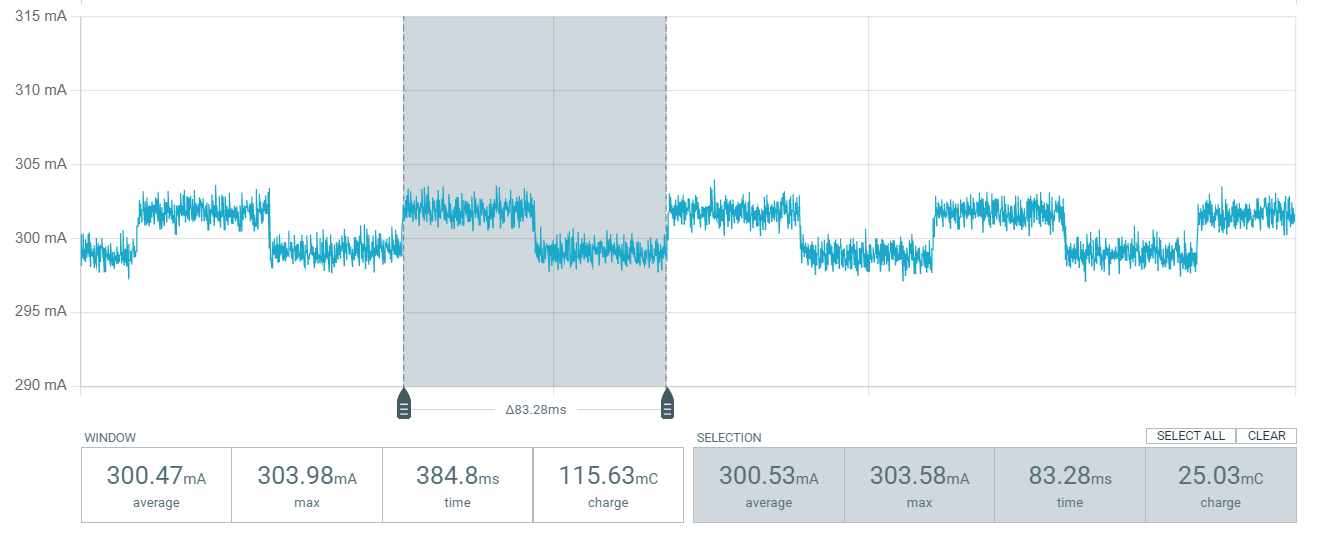
\includegraphics[width=0.9\textwidth]{Images/PPK_ping_zoom.png}
    \caption[Zoomed in current consumption for ICMP pings]{Zoomed in current consumption for ICMP pings.}
    \label{fig:ppk_icmp_ping}
\end{figure}



The next test was done when accessing the webserver. Figure \ref{fig:ppk_http_annotated} shows 5 different regions where each region is a result of a different action. The left most tests is from the inital HTTP requests to get the index page. Notably, there is 2 separate sections here, this is because the client fetches the html, css and favicon first and then requests the main (and much larger) javascript file after. The readings for each of these points is given as: average current, maximum current and time going from top to bottom. 

The second test is what happens when you click to navigate to the about page. The third event is when navigating to the config page and the 4th event is what happens when you press the 'load rules' button. The final test case is a refresh on the main page for the statistics. Notably, as the javascript (thus client) is doing the routing and page handling, future requests to get the contents of the pages are not needed, but only small API requests to update the data. Coincidentally, these first 3 requests also trigger a SD card read and explains the higher current draw. The fourth request also creates a read request to the SD card, but only needs to read a single page. The fifth request does not involve a read or write to the SD card, but rather just a simple SPI transaction takes place and consequently doesn't draw much additional power. 

\begin{figure}[h]
    \centering
    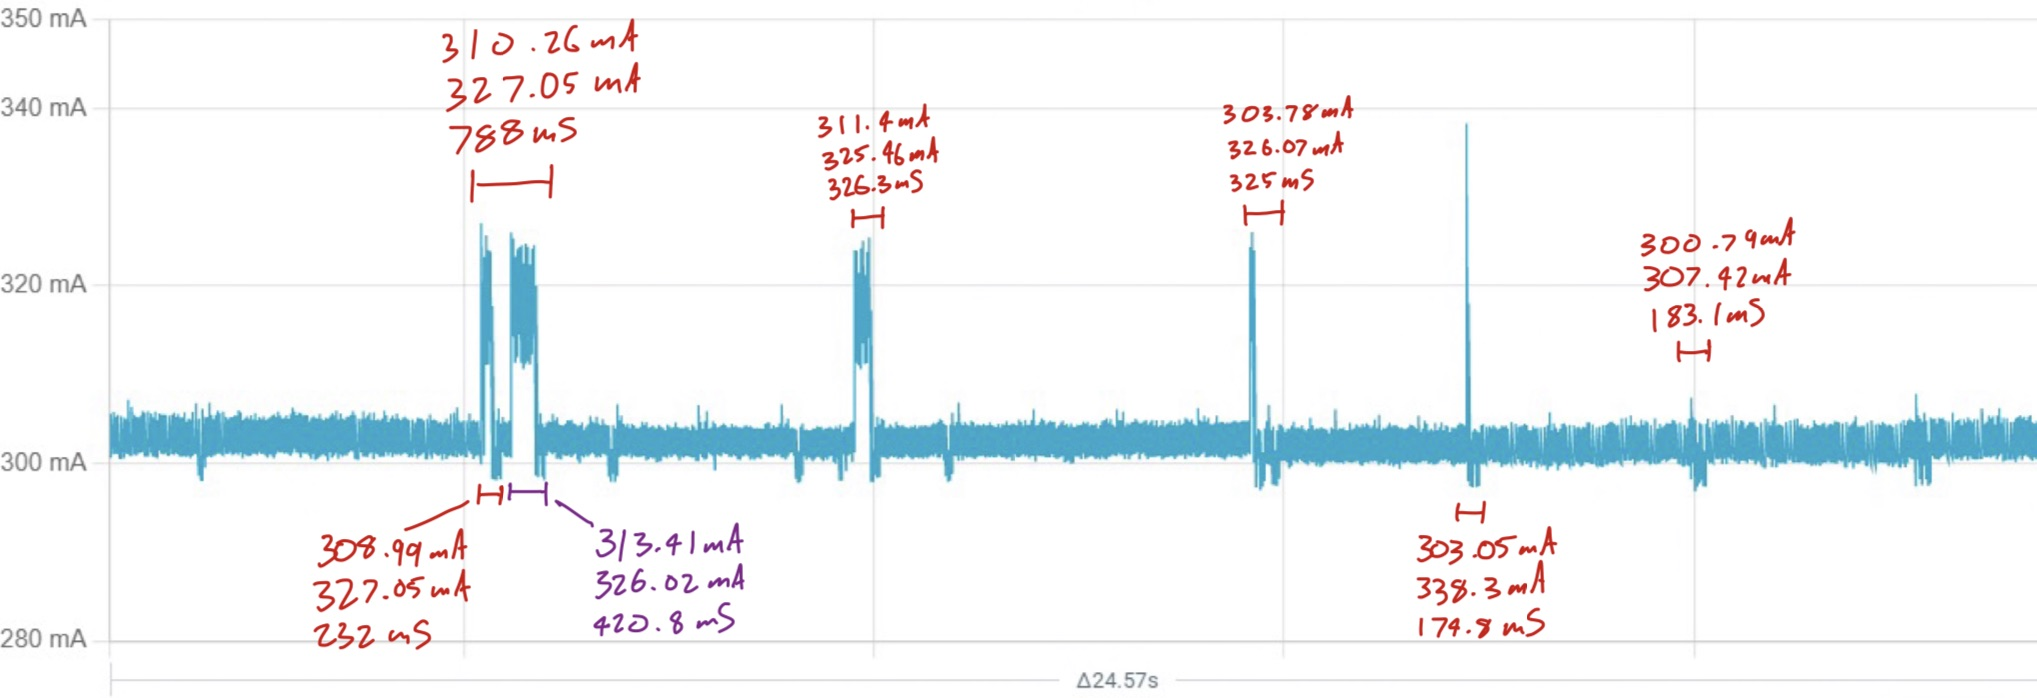
\includegraphics[width=0.9\textwidth]{Images/PPK_http_annotated.png}
    \caption[Current consumption of FPGA board with HTTP requests]{Current consumption of FPGA board with HTTP requests.}
    \label{fig:ppk_http_annotated}
\end{figure}




% HOW TO ADD ADDITIONAL CHAPTERS
% Step One: Add a new folder called "ChapterX" (X being the chapter number).
% Step Two: Within the folder add a new .tex file by clicking the "New File" button in the Overleaf Menu. Rename the file to a title of your choice.
% Step Three: Copy the Chapter 2 headline and "\input" command located above and insert it below Chapter 2.
% Step Four: Rename the headline to your specific chapter number, change the input command to include the name of the folder you created and the name of the file you created.
% Repeat this process for every chapter.

%CONCLUSION CHAPTER
% ***************************************************
% Conclusion
% ***************************************************
\chapter[Conclusion]{Conclusion}
\label{Chap:Conclusion}

% ********* Enter your text below this line: ********
Conclude your thesis.

% ***************************************************

% ***************************************************
% Bibliography
%****************************************************
%CHOOSE YOUR BIB STYLE AND FILE.
%We have included the following two referencing styles for you to use in your thesis. You can add an alternate style if you prefer.

%Style: apalike = this is an (Author, Year) referencing style similar to APA
%Style: elsarticle-num = this is a numbered referencing style that will display the bibliography in citation order

%To use one of the styles provided ensure the % is removed from the start of the line, and the other option is commented out with a % at the start of the line. The style elsarticle-num is active by default.

%\bibliographystyle{apalike}
\bibliographystyle{ieeetr}

\bibliography{./References/Bibliography}


%When you have finished your thesis we recommend that you manually fix any errors in your bibliography. 
%To do this, compile, copy the .bbl into a new .tex file and include this here after commenting out the other bibliography commands. Make corrections in that .tex file.

% ***************************************************
% Appendices
%**************************************************** 
%UNCOMMENT THIS SECTION IF YOU ARE USING APPENDICES.
%Simply adapt the same formatting used for other chapters.
\appendix
% If you need appendix in your thesis then consider the following appendix file (you can add more if you need more) otherwise you should not consider it in your main thesis.
% ***************************************************
% Appendix
% ***************************************************
\chapter{Appendix}

Write your appendix here. Following two are examples. 


\section{Neorv32 memory address space layout}
\label{app:mem_address}
\begin{figure}[h!]
    \centering
    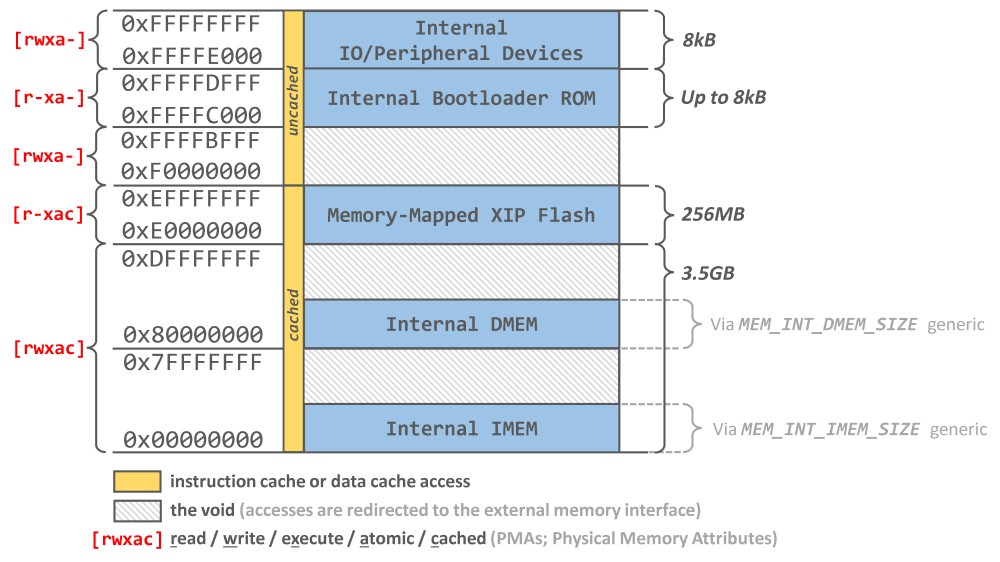
\includegraphics[width=1\textwidth]{Images/neorv32_address_space.png}
    \caption{Neorv32 Memory Address space.}
\end{figure}



\section{FPGA primitives utilisation}
\label{app:res_usage}
\begin{table}
    \centering
    \caption{FPGA primitives utilisation for XC7A100T}
    \begin{tabular}{|l|r|l|}
        \toprule
        Ref Name   & Used & Functional Category \\
        \midrule
        LUT6       & 16262 & LUT \\
        LUT5       & 14820 & LUT \\
        FDRE       & 14500 & Flop \& Latch \\
        LUT3       & 13222 & LUT \\
        MUXF7      &  2436 & MuxFx \\
        FDCE       &  1875 & Flop \& Latch \\
        RAMD64E    &  1836 & Distributed Memory \\
        LUT4       &  1294 & LUT \\
        LUT2       &  1016 & LUT \\
        MUXF8      &   884 & MuxFx \\
        CARRY4     &   437 & CarryLogic \\
        LUT1       &   156 & LUT \\
        RAMB36E1   &   130 & Block Memory \\
        FDPE       &    41 & Flop \& Latch \\
        OBUF       &    40 & IO \\
        LDCE       &    36 & Flop \& Latch \\
        IBUF       &    24 & IO \\
        SRLC32E    &    21 & Distributed Memory \\
        OBUFT      &    11 & IO \\
        BUFG       &     8 & Clock \\
        FDSE       &     5 & Flop \& Latch \\
        DSP48E1    &     4 & Block Arithmetic \\
        SRL16E     &     1 & Distributed Memory \\
        MMCME2\_ADV &    1 & Clock \\
        \bottomrule
    \end{tabular}
\end{table}

\begin{table}
    \centering
    \caption{Memory Utilisation}
    \begin{tabular}{|l|r|r|r|r|r|}
        \toprule
        Site Type      & Used & Fixed & Prohibited & Available & Util\% \\
        \midrule
        Block RAM Tile &  130 &     0 &          0 &       135 & 96.30 \\
        RAMB36/FIFO*   &  130 &     0 &          0 &       135 & 96.30 \\
        RAMB36E1 only  &  130 &     - &          - &         - &    -  \\
        RAMB18         &    0 &     0 &          0 &       270 &  0.00 \\
        \bottomrule
    \end{tabular}
\end{table}

\begin{table}
    \centering
    \caption{Slice Logic Utilisation}
    \begin{tabular}{|l|r|r|r|r|r|}
        \toprule
        Site Type                 & Used & Fixed & Prohibited & Available & Util\% \\
        \midrule
        Slice LUTs*               & 40920 &     0 &          0 &     63400 & 64.54 \\
        LUT as Logic              & 39062 &     0 &          0 &     63400 & 61.61 \\
        LUT as Memory             &  1858 &     0 &          0 &     19000 &  9.78 \\
        LUT as Distributed RAM    &  1836 &     - &          - &         - &    -  \\
        LUT as Shift Register     &    22 &     - &          - &         - &    -  \\
        Slice Registers           & 16457 &     0 &          0 &    126800 & 12.98 \\
        Register as Flip Flop     & 16421 &     0 &          0 &    126800 & 12.95 \\
        Register as Latch         &    36 &     0 &          0 &    126800 &  0.03 \\
        F7 Muxes                  &  2436 &     0 &          0 &     31700 &  7.68 \\
        F8 Muxes                  &   884 &     0 &          0 &     15850 &  5.58 \\
        \bottomrule
    \end{tabular}
\end{table}



% ***************************************************
% Back Matter
%**************************************************** 
%COMMENT OUT IF YOU DO NOT WISH TO INCLUDE BACK MATTER.
% % ***************************************************
% Back Matter
% ***************************************************
% ADD AN ENDQUOTE HERE. If you do not wish to, delete this file.
\backmatter

\normalfont
\cleartooddpage

\pagestyle{empty}

\begin{table}[b!]
\begin{center}
% ********* Enter your quote within {} brackets: ********
\textit{Endquote goes here.}

% ********************************************************
\end{center}
\begin{flushright}
% ********* Enter your text below, as indicated: ********
Author of quote,\\
Source of quote

% ********************************************************
\end{flushright}
\end{table}

\end{document}
